% load packages
\documentclass{article}
\usepackage[english]{babel}
\usepackage[utf8]{inputenc}
\usepackage{johd}

\title{Forecasting Air Cargo Demand for Southeast Asia}

\author{Josephine Tan Xin Yi$^{a}$, Michael Hoon Yong Hau$^{a}$\\
        \small $^{a}$Singapore University of Technology and Design, Singapore \\\\
        \small \textbf{Principal Investigator}: Peter Jackson$^{b}$, \textbf{Project Lead}: Jamie Bloomfield$^{b}$ \\
        \small $^{b}$Aviation Studies Institute, Singapore University of Technology and Design, Singapore \\
}

\date{$3\textsuperscript{rd}$ January $2023$} %leave blank

\begin{document}

\maketitle

\begin{figure}[t!]
    \centering
    
\includegraphics[width=0.2\textwidth]{images/ASI Graphics/sutd-asi-logo-web-2021-fc.png}
    
\includegraphics[width=0.2\textwidth]{images/ASI Graphics/asi-logo-web-2022-fc.png}
    
\includegraphics[width=0.2\textwidth]{images/ASI Graphics/asi-logo-web-2021-fc-02-v2.png}
    \label{titlefig}
\end{figure}

\begin{abstract} 
\noindent The demand for air freight within ASEAN countries is influenced by a range of macroeconomic factors. These factors can include economic growth, consumer spending, exchange rates, and trade policies. Trade policies, such as tariffs or other barriers to trade, can also affect the demand for air freight within ASEAN countries. Changes in trade policies can lead to changes in the flow of goods between countries and therefore the demand for air freight. Overall, the demand for air freight within ASEAN countries is influenced by a complex mix of economic and trade-related factors. Understanding these factors can help companies and policymakers to anticipate and respond to changes in the demand for air freight in the region.
\end{abstract}

\noindent\keywords{Air Freight Demand; Air Cargo; Forecasting; Southeast Asia}

\newpage

\tableofcontents

\newpage

\section{Introduction}

\subsection{Objective}

This project is performed under the Undergraduate Research Opportunities Programme (UROP) at the Singapore University of Technology and Design (SUTD) and supervised through the Aviation Studies Institute (ASI). This programme provides university students with the opportunity to apply research techniques as part of their undergraduate studies for short duration projects (up to c. 3-months). \\

\noindent The project objective is to support the prediction of future air cargo demand within Southeast Asia by identifying the factors of significance and reliable open-source data. It leverages confidential historical air cargo demand data supplied by an external organisation (International Air Transport Association, [IATA]) who are collaborating with ASI. \\

\noindent The work would be the first step in developing applied insights of direct relevance to the air transport industry. \\

\subsection{Motivation}

Air Cargo has grown in relevance during the COVID-19 pandemic as a means to transport perishable goods in a timely manner. Despite extensive data on historical air cargo demand, predicting future demand remains poorly defined. Whilst passenger air transport demand is understood to have a general correlation with Gross Domestic Product (GDP) \cite{GDPcorr}, several other macroeconomic factors are thought to play a pivotal role in air cargo demand. The specific factors are thought to vary in different geographical regions. \\

\noindent This project involved identifying factors of significance for predicting air cargo demand within the Southeast Asia region over long-time horizons. \\

\noindent The work uses extensive historical data related to air cargo demand (obtained from the IATA CargoIS platform), open-source macroeconomic data (historical and forecast) and data models to search for correlations. \\

\noindent A second challenge was to develop mathematical models that searched for correlations between the acceptable macroeconomic data and the historical air cargo demand. These were used to identify the factors of significance when predicting future air cargo demand in the region. 

\section{Analysis of Air Cargo Demand}

After obtaining the relevant air cargo dataset from IATA in Comma Separated Values (CSV) format, DBeaver was used as a relational database management system (RDBMS) to manage the provided data. SQLite was used as our main language to query the required data. \\

\noindent The initial dataset provided by IATA's CargoIS platform ranged monthly from January 2015 to December 2018, and included each origin country's total weight and number of shipments to each receiving country.


\subsection{Data Cleaning and Management}

As the scope of our project involves analysis of air cargo demand within Asia, we have decided to focus on analysis between ASEAN countries within the Southeast Asia region. This significantly narrows down and reduces the size of the dataset, for easier identification of relevant correlations with macroeconomic data. \\

\noindent Due to data availabilities, we initially sourced and collated a multitude of macroeconomic and non-macroeconomic datasets for each country from open-source resources. Open-source datasets were generally available on an annual basis and we obtained these across $\sim60$ years ($1960 - 2021$, provided by World Bank Data) to aid multi-year time series correlation analysis. \\

\noindent We subsequently obtained the historical air cargo data, which was provided on a monthly basis. However, we realised that this range was limited from 2015 to 2018. This meant that there would be only four available data points if analysing on an annual basis. As this would be insufficient for any meaningful analysis (low sample sizes would not produce credible results), we investigated the availability of further macroeconomic datasets. We were able to obtain quarterly datasets for GDP, from the central banks and monetary authorities (and their equivalents) of 6 ASEAN countries. \\

\noindent As a consequence, we aggregated each year's worth of air cargo data into quarterly totals. This would bring us to a total of 16 data points per country, which was enough to show potential trends and seasonality in the data. \\

\noindent Our second challenge while working with the historical air cargo data was that the different countries had naturally vastly different number of shipments and monthly weights, by virtue of their differing levels of economic development. This resulted in a relatively high sample standard deviation across the ASEAN region, which made it difficult to perform comparative analysis of the raw data. To overcome this issue, we employed feature scaling techniques on the raw data, namely base 10 logarithmic scaling, to better visualise the data in maps and radar charts. 

\subsection{Exploratory Data Analysis}

\subsubsection{Air Cargo Trade Relations}

Initial analysis was performed using \textit{R} code in \textit{RStudio} to visualise the key geographical flows of air freight between ASEAN countries. This was done by combining our current dataset with \href{https://github.com/google/dspl}{open-source geospatial data} from Google, which contained longitude and latitude coordinates representing each country. Due to limitations of the dataset, this geospatial plot does not represent the exact take-off and landing coordinates of each flight, nor of the flight paths taken by aircraft. \\ 

\noindent Air cargo shipment activity between each ASEAN state, aggregated from 2015 to 2018, is shown below. The thickness of each line indicates the relative number of exports from each country. \\

\begin{subfigures}
\begin{figure}[H]
    \centering
    \subfloat[\centering Singapore's Aggregated Exports]{{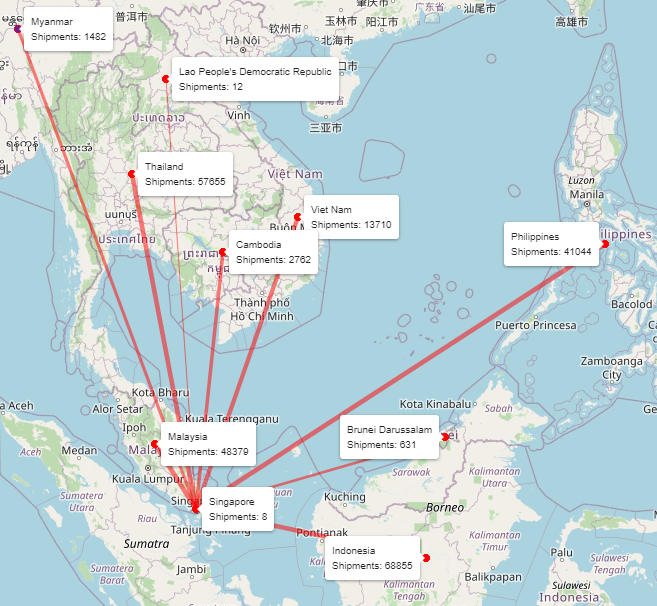
\includegraphics[width=0.475\textwidth]{images/Map Visualisations/Singapore_Exports.png}}}
    \qquad
    \subfloat[\centering Malaysia's Aggregated Exports]{{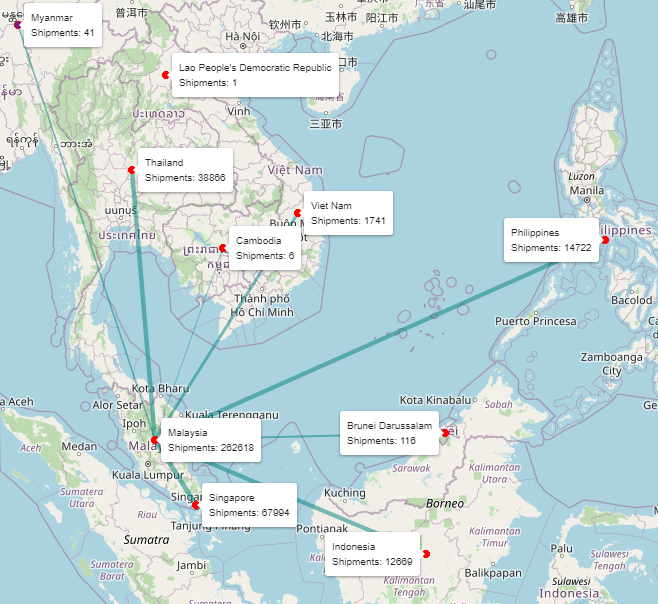
\includegraphics[width=0.475\textwidth]{images/Map Visualisations/Malaysia_Exports.png}}}
    \qquad
    \subfloat[\centering Thailand's Aggregated Exports]{{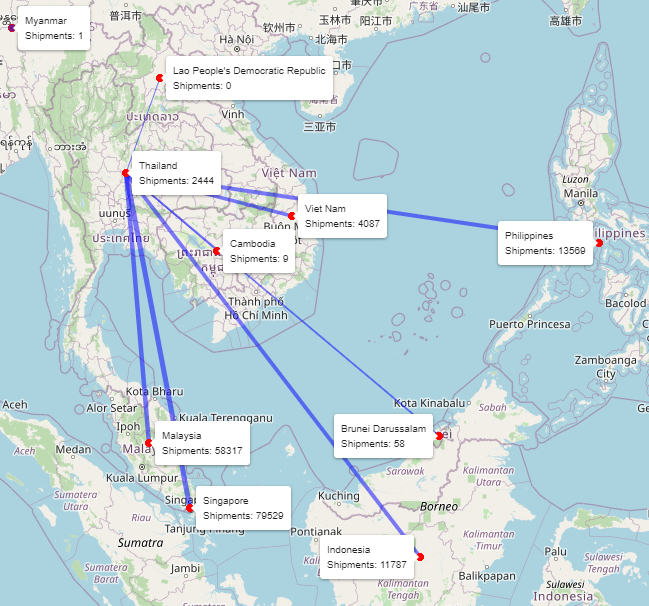
\includegraphics[width=0.475\textwidth]{images/Map Visualisations/Thailand_Exports.png}}}
    \qquad
    \subfloat[\centering Vietnam's Aggregated Exports]{{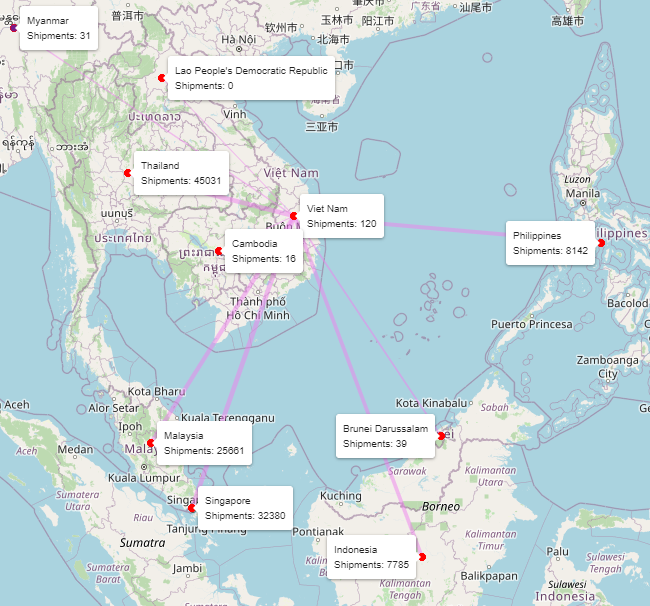
\includegraphics[width=0.475\textwidth]{images/Map Visualisations/Vietnam_Exports.png}}}
    \qquad
    \subfloat[\centering Philippines's Aggregated Exports]{{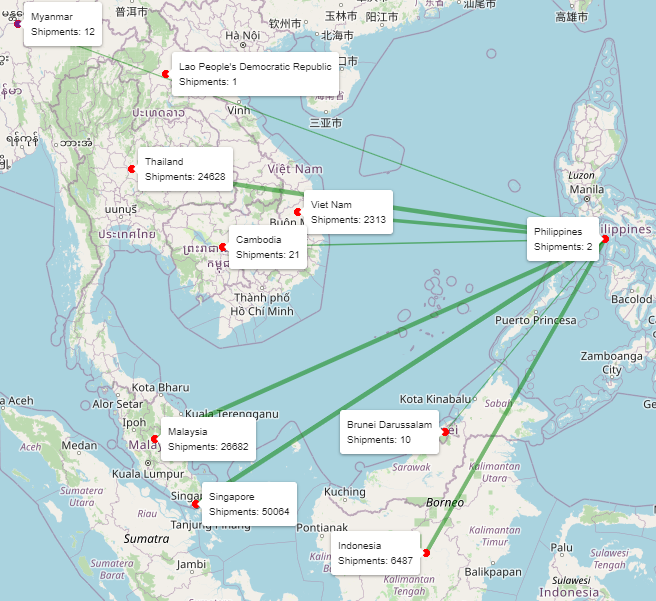
\includegraphics[width=0.475\textwidth]{images/Map Visualisations/Philippines_Exports.png}}}
    \qquad
    \subfloat[\centering Brunei's Aggregated Exports]{{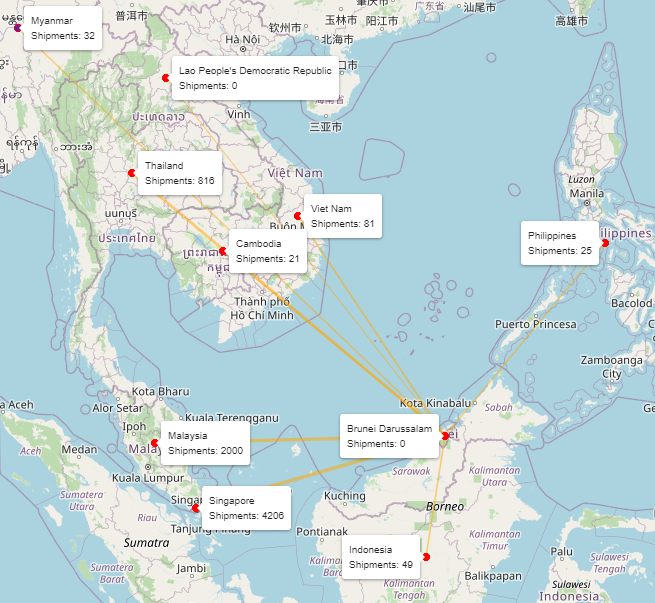
\includegraphics[width=0.475\textwidth]{images/Map Visualisations/Brunei_Exports.png}}}
    \caption{Aggregated Exports to ASEAN (2015 to 2018)}
\end{figure}
\begin{figure}[H]
    \centering
    \subfloat[\centering Cambodia's Aggregated Exports]{{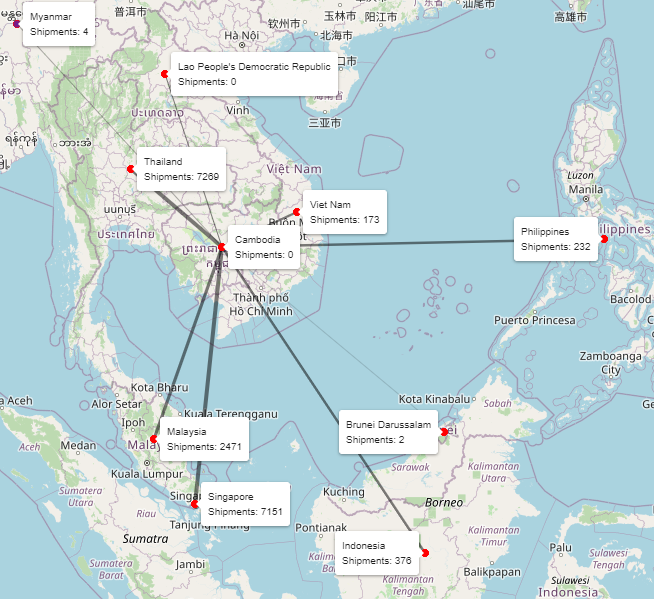
\includegraphics[width=0.475\textwidth]{images/Map Visualisations/Cambodia_Exports.png}}}
    \qquad
    \subfloat[\centering Laos' Aggregated Exports]{{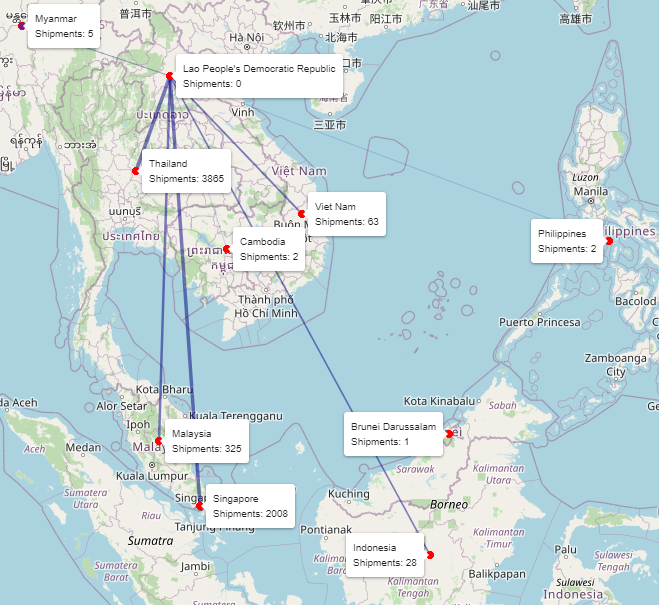
\includegraphics[width=0.475\textwidth]{images/Map Visualisations/Laos_Exports.png}}}
    \qquad
    \subfloat[\centering Indonesia's Aggregated Exports]{{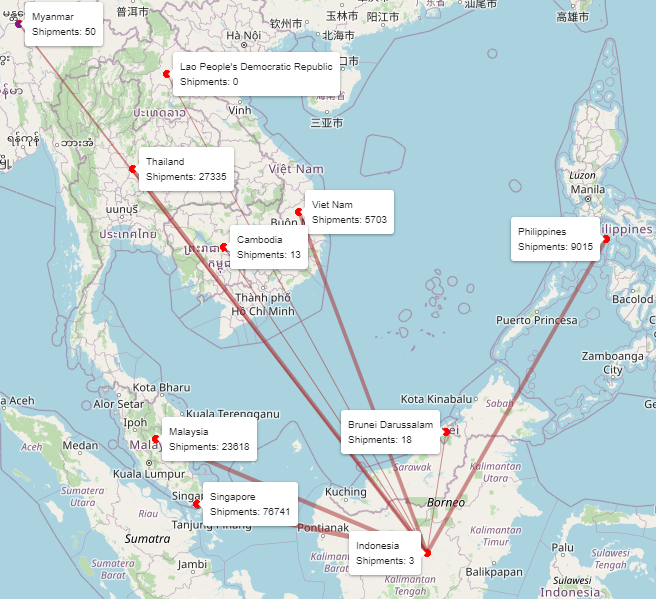
\includegraphics[width=0.475\textwidth]{images/Map Visualisations/Indonesia_Exports.png}}}
    \qquad
    \subfloat[\centering Myanmar's Aggregated Exports]{{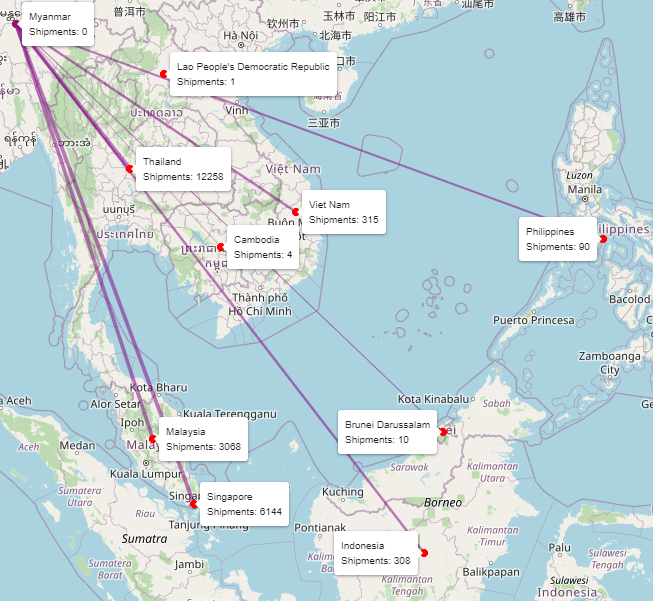
\includegraphics[width=0.475\textwidth]{images/Map Visualisations/Myanmar_Exports.png}}}
    \caption{Aggregated Exports to ASEAN (2015 to 2018)}
\end{figure}
\end{subfigures}

\noindent Some key observations can be observed from the geospatial visualisation: \\

\begin{itemize}
    \item Laos has one of the lowest air cargo activities amongst all the ASEAN countries. Despite exporting to many countries, it does not seem to receive a corresponding quantity of imports (interestingly, Laos is the only land-locked country in Southeast Asia). 
    \item Different countries have different major trading partners for air cargo, although Singapore, Malaysia, and Thailand have particularly high proportions of air cargo shipment activity with other ASEAN countries regardless.
    \item Malaysia has a disproportionately large domestic air cargo shipment activity compared to other countries. The exact origin and destination of domestic air cargo is not known due to the lack of information in the dataset.
\end{itemize}

\newpage

\subsubsection{Annual Imports of Air Cargo Per Country}

Interactive radar charts were generated in \textit{Python} code, with options to display the years as coloured overlays. The radar charts give an additional overview of the interaction between the ASEAN countries, which in this case represents the total number of imports per year. The number of shipments have been log-scaled, and as such the axis represents the scaled value of shipments, i.e. number of shipments $= 10^r$, with $r$ being the value on the axis. \\

\noindent We are also able to visualise and compare each country's internal shipments with that of other countries, as well as countries with no interaction between one another. The legend of the chart is as follows: blue representing 2015, red representing 2016, green representing 2017, and purple representing 2018. \\

\begin{subfigures}
\begin{figure}[H]
    \centering
    \subfloat[\centering Singapore's Annual Imports]{{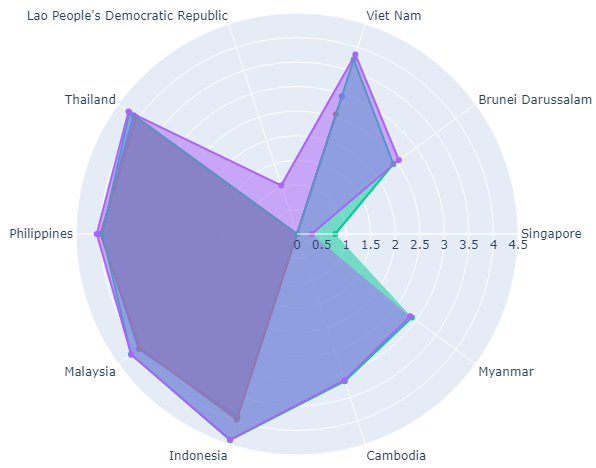
\includegraphics[width=0.475\textwidth]{images/Radar Plots/Singapore_Radar.png}}}
    \qquad
    \subfloat[\centering Malaysia's Annual Imports]{{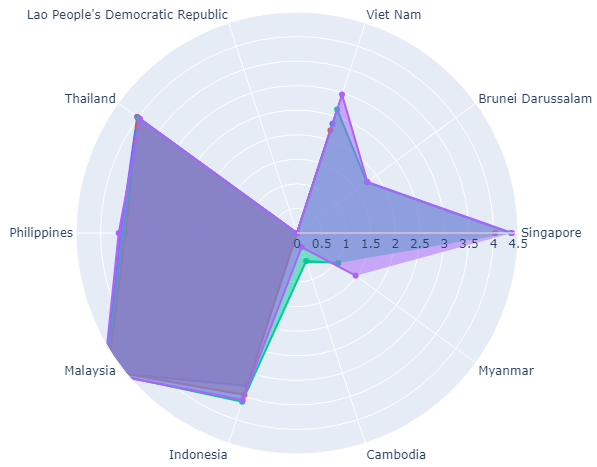
\includegraphics[width=0.475\textwidth]{images/Radar Plots/Malaysia_Radar.png}}}
    \qquad
    \subfloat[\centering Thailand's Annual Imports]{{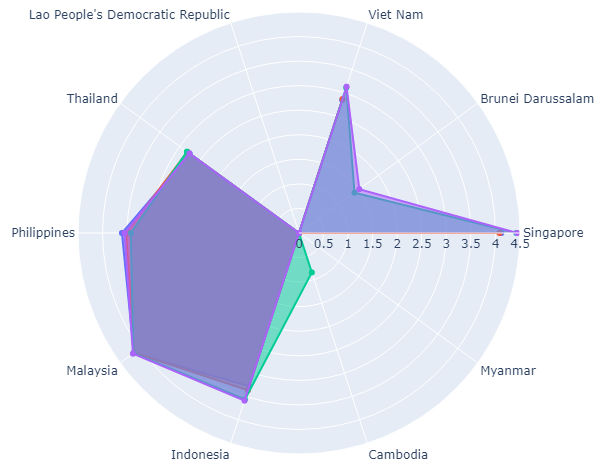
\includegraphics[width=0.475\textwidth]{images/Radar Plots/Thailand_Radar.png}}}
    \qquad
    \subfloat[\centering Vietnam's Annual Imports]{{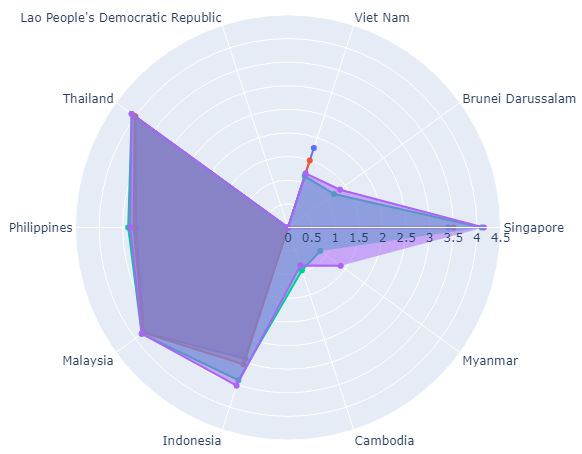
\includegraphics[width=0.475\textwidth]{images/Radar Plots/Vietnam_Radar.png}}}
    \caption{Aggregated Imports to ASEAN (2015 to 2018)}
\end{figure}

\begin{figure}[H]
    \centering
    \subfloat[\centering Philippines's Annual Imports]{{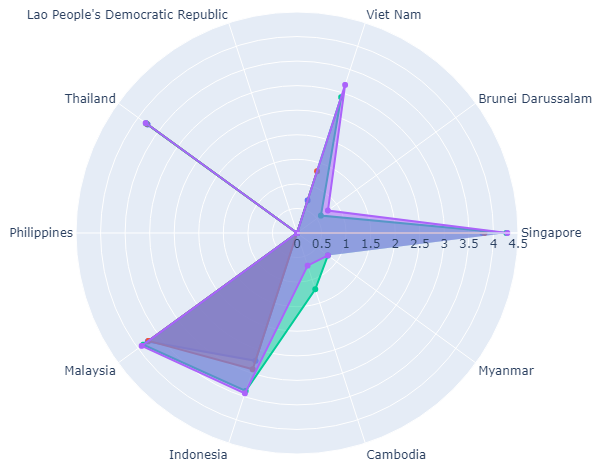
\includegraphics[width=0.475\textwidth]{images/Radar Plots/Philippines_Radar.png}}}
    \qquad
    \subfloat[\centering Brunei's Annual Imports]{{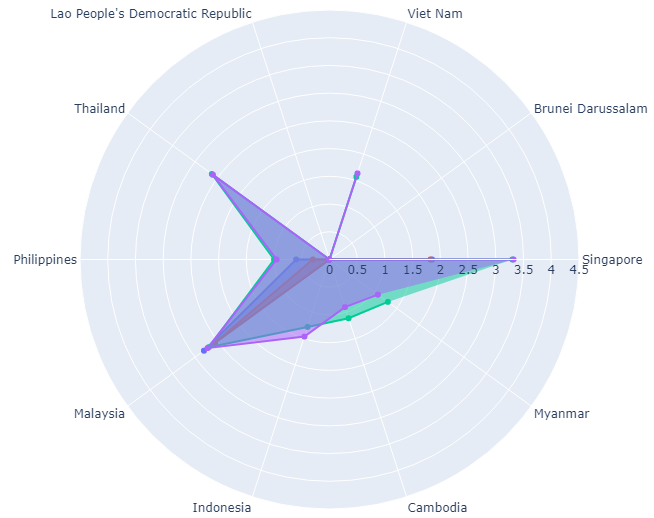
\includegraphics[width=0.475\textwidth]{images/Radar Plots/Brunei_Radar.png}}}
    \qquad
    \subfloat[\centering Cambodia's Annual Imports]{{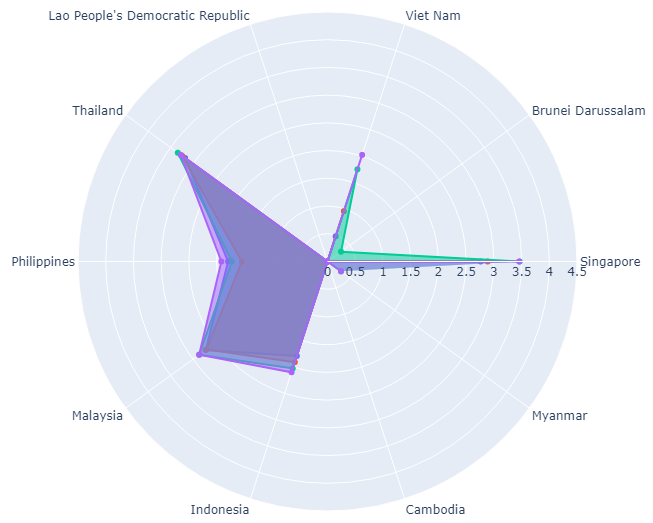
\includegraphics[width=0.475\textwidth]{images/Radar Plots/Cambodia_Radar.png}}}
    \qquad
    \subfloat[\centering Laos' Annual Imports]{{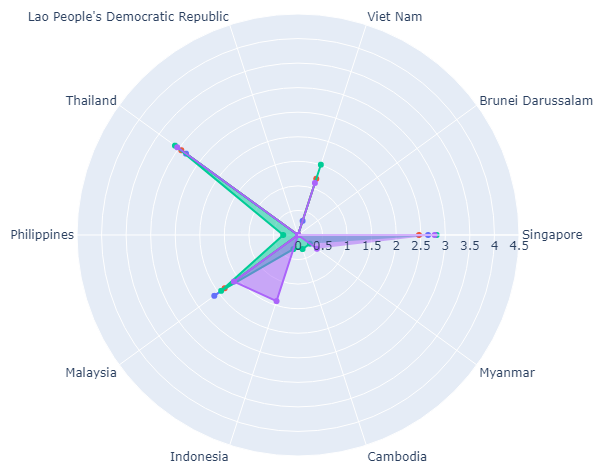
\includegraphics[width=0.475\textwidth]{images/Radar Plots/Lao_Radar.png}}}
    \qquad
    \subfloat[\centering Indonesia's Annual Imports]{{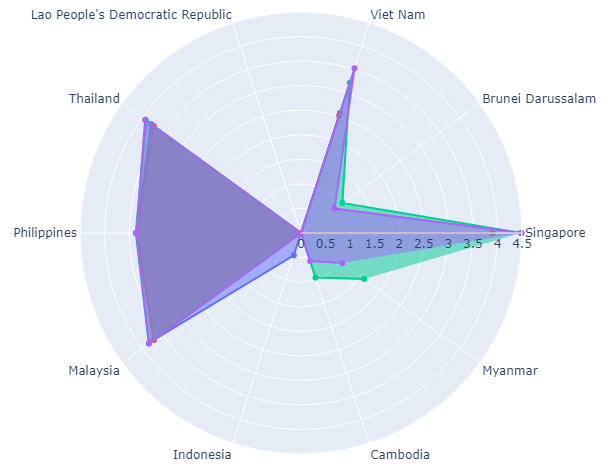
\includegraphics[width=0.475\textwidth]{images/Radar Plots/Indonesia_Radar.png}}}
    \qquad
    \subfloat[\centering Myanmar's Annual Imports]{{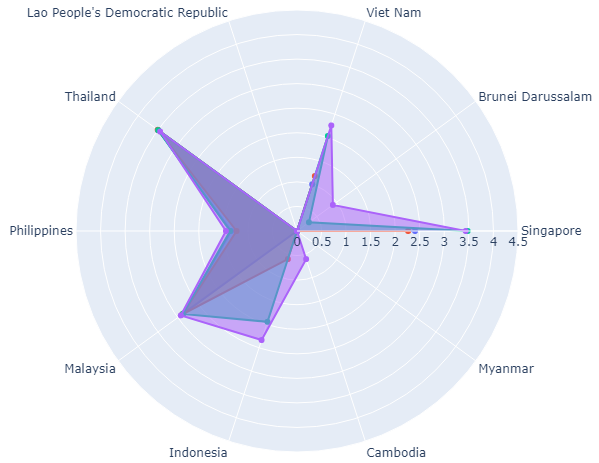
\includegraphics[width=0.475\textwidth]{images/Radar Plots/Myanmar_Radar.png}}}
    \caption{Aggregated Imports to ASEAN (2015 to 2018)}
\end{figure}
\end{subfigures}

\newpage

\noindent Some interesting analysis to note: \\

\begin{itemize}
    \item While most countries do not import from themselves, Malaysia seems to once again have a disproportionately high number of internal air cargo shipments. 
    \item There seems to be a noticeable jump in the number of imports from 2016 to 2017, which is consistent for all countries. The number of imports from 2015 to 2016 and from 2017 to 2018 stays relatively consistent, however.
    \item The disproportionate increase in trade between countries from 2016 to 2017 might be due to more countries participating in the ASEAN Free Trade Area (AFTA). The AFTA was signed at the 1992 ASEAN Summit in Singapore. Its objectives include the elimination and reduction of import duties, removal of Non-Tariff Barriers (NTBs), among many others, aimed at creating a robust intra-ASEAN trade. It was not until 2015 however, that the AFTA achieved, among others, eliminating tariffs and facilitating trade between countries \cite{asean2}.
\end{itemize}

\newpage

\subsubsection{Quarterly Air Freight Demand}
The following figures depict line charts, displaying the amount of shipment activity (total imports and exports) for each country within the ASEAN region. The plots are separated into two, with one including the countries with higher shipment activity, and the other with lower shipment activity. This allows for better visual comparison between countries with vastly different shipment activity, to identify commonalities in trends.

\begin{subfigures}
    \begin{figure}[H]
        \centering
        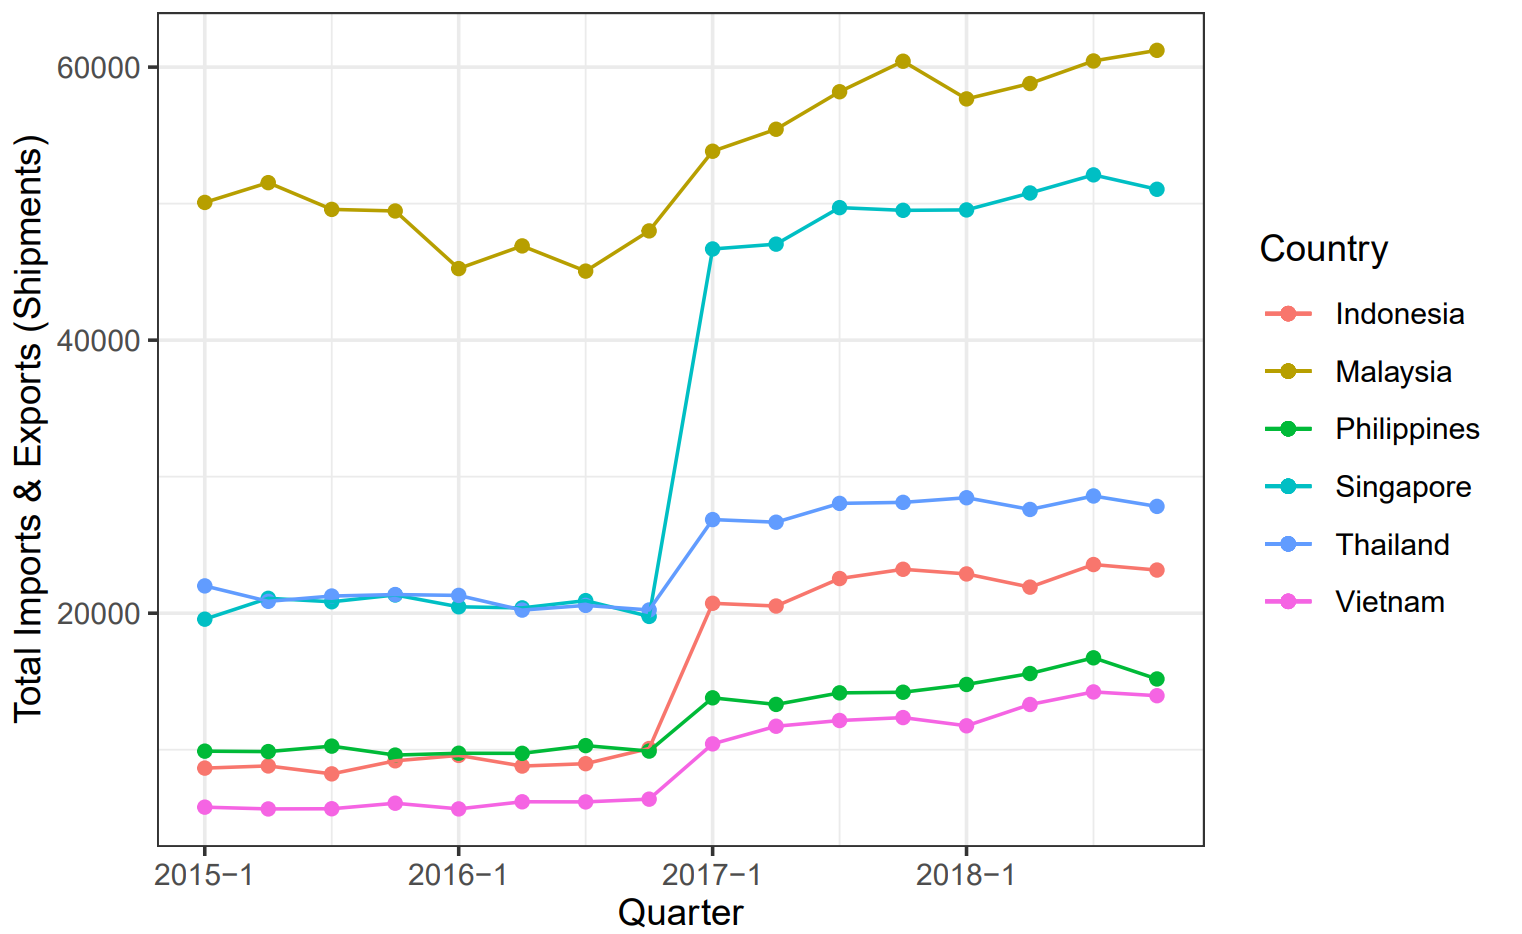
\includegraphics[width=1\textwidth]{images/Line Plots/ASEAN/ASEAN_Large_Quarterly_Shipments_BigFont.png}
        \caption{\label{fig2}Total Shipments for Larger Activity Countries}
    \end{figure}
    
    \begin{figure}[H]
        \centering
        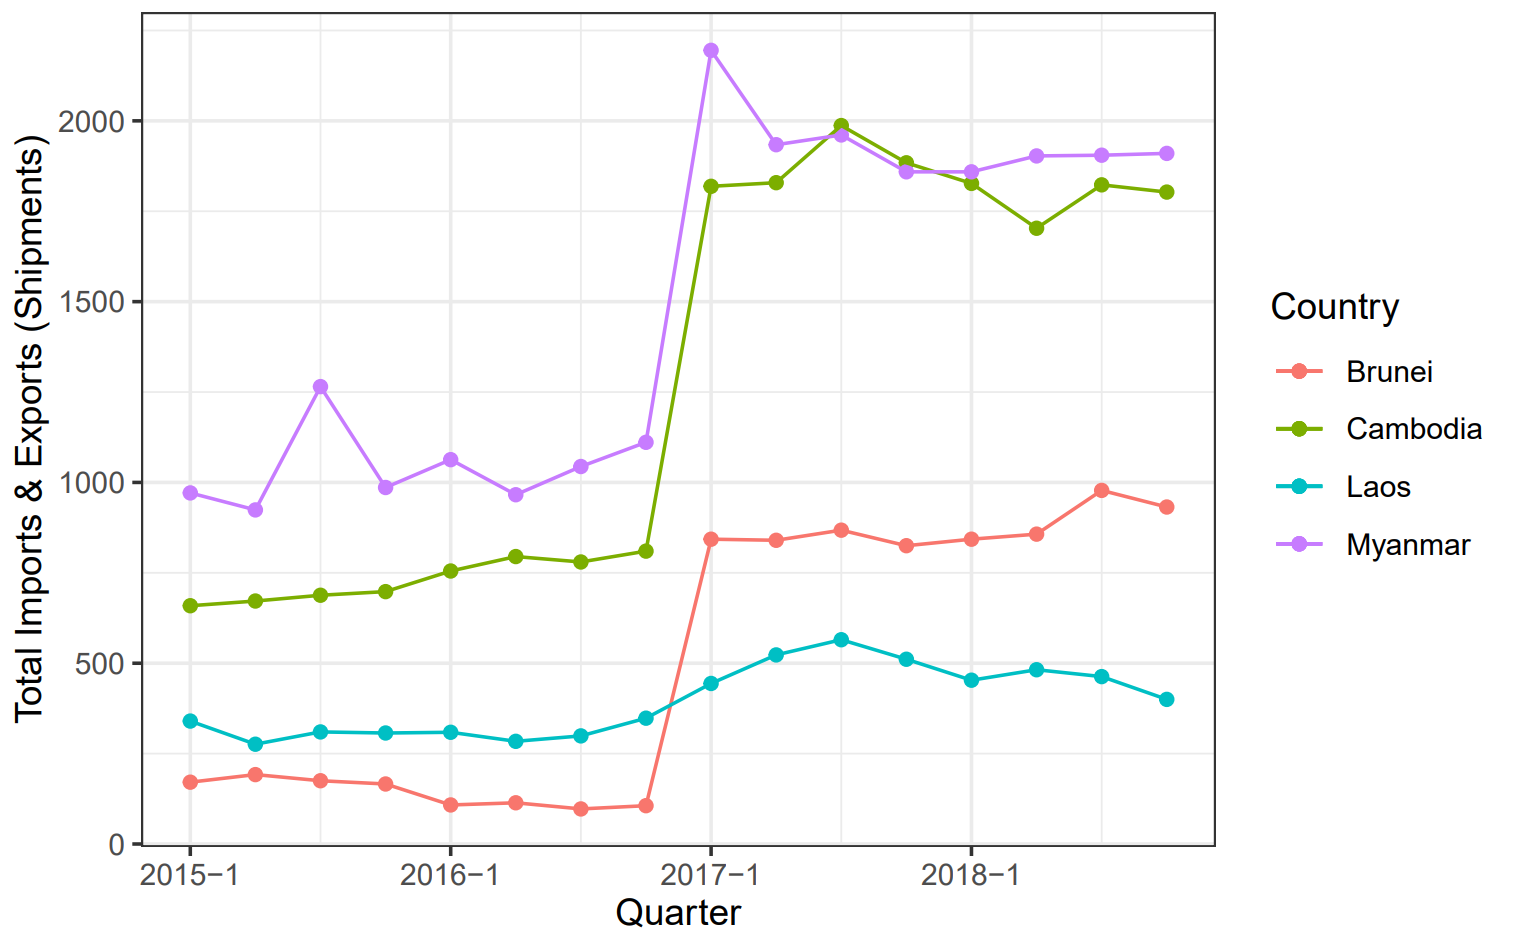
\includegraphics[width=1\textwidth]{images/Line Plots/ASEAN/ASEAN_Small_Quarterly_Shipments.png}
        \caption{\label{fig2}Total Shipments for Smaller Activity Countries}
    \end{figure}
\end{subfigures}

\noindent Similarly, there is a large increase in the number of shipments from 2016 Q4 to 2017 Q1 for most countries. The only exception to this trend is Laos, where the change in shipment over time seems to be comparatively gradual rather than sudden.

\subsubsection{Seasonal Trend Analysis}
The line plots below depict the monthly data for the aggregated number of shipments (Imports and Exports) for each country, showing a slight seasonal trend during the months of March to April and October to November. We have included both the logarithmic-scaled plots and the raw data plots, as the raw data plots show a better visualisation of seasonal trends, but obscure the countries with lower activity. The scaled plots thus supplement the visualisation of the countries with lower air cargo activity.

\newpage

\begin{figure}[H]
    \begin{minipage}[c]{1\linewidth}
        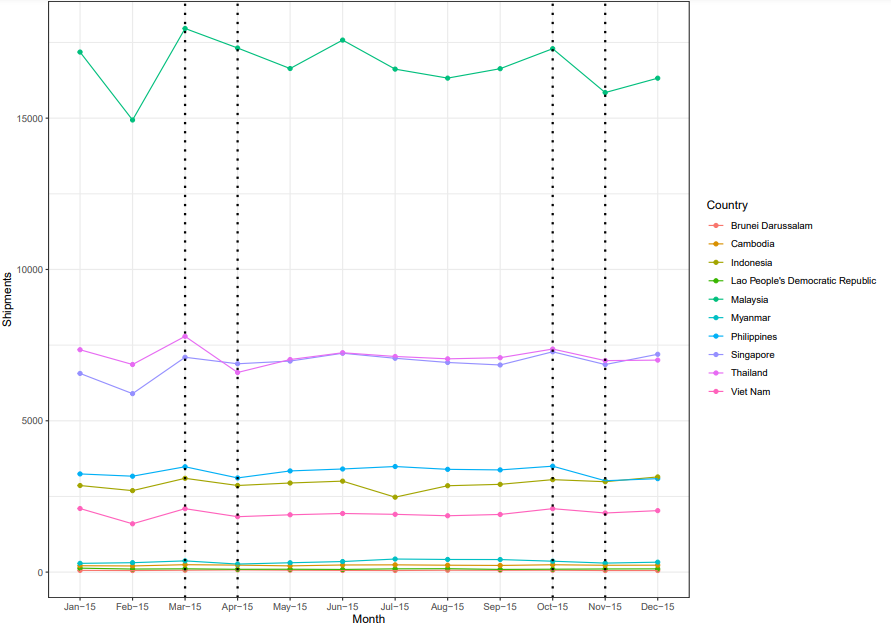
\includegraphics[width=\linewidth]{images/Line Plots/Seasonal/2015_seasonal.png}
    \end{minipage}
    \hfill
    \begin{minipage}[c]{1\linewidth}
        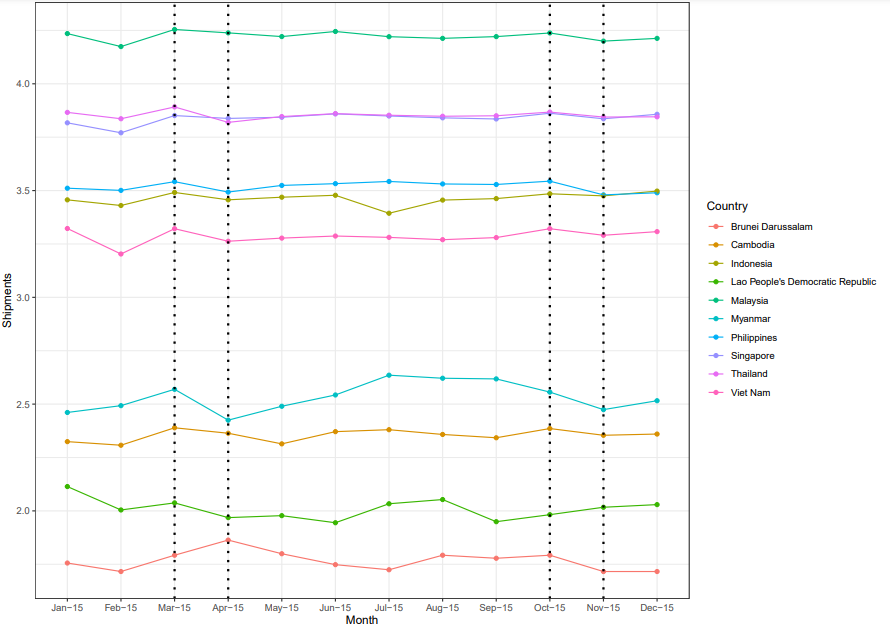
\includegraphics[width=\linewidth]{images/Line Plots/Seasonal/2015_seasonal_log.png}
        \caption{2015 Monthly Shipments, regular and log-scaled (below)}
    \end{minipage}
\end{figure}

\begin{figure}[H]
    \begin{minipage}[c]{1\linewidth}
        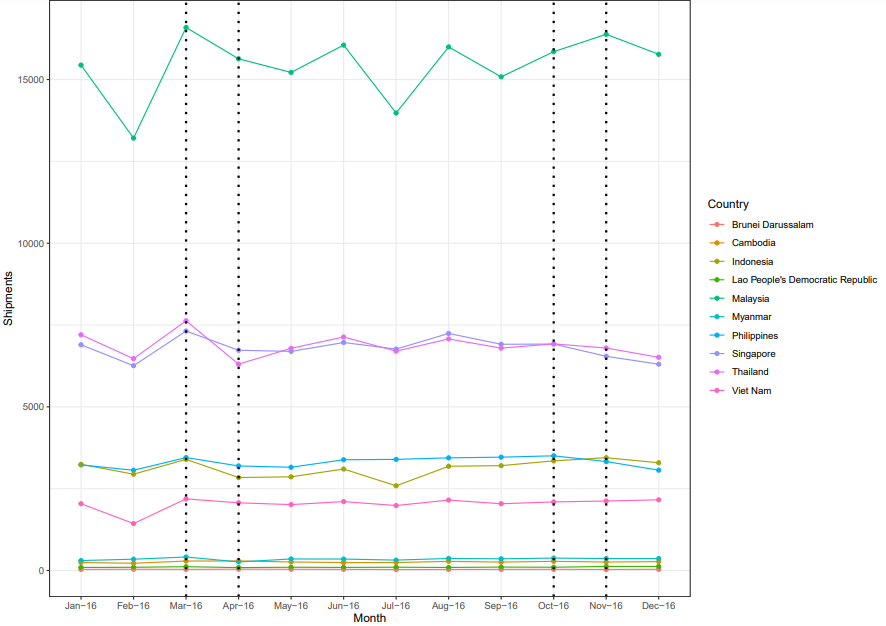
\includegraphics[width=\linewidth]{images/Line Plots/Seasonal/2016_seasonal.png}
    \end{minipage}
    \hfill
    \begin{minipage}[c]{1\linewidth}
        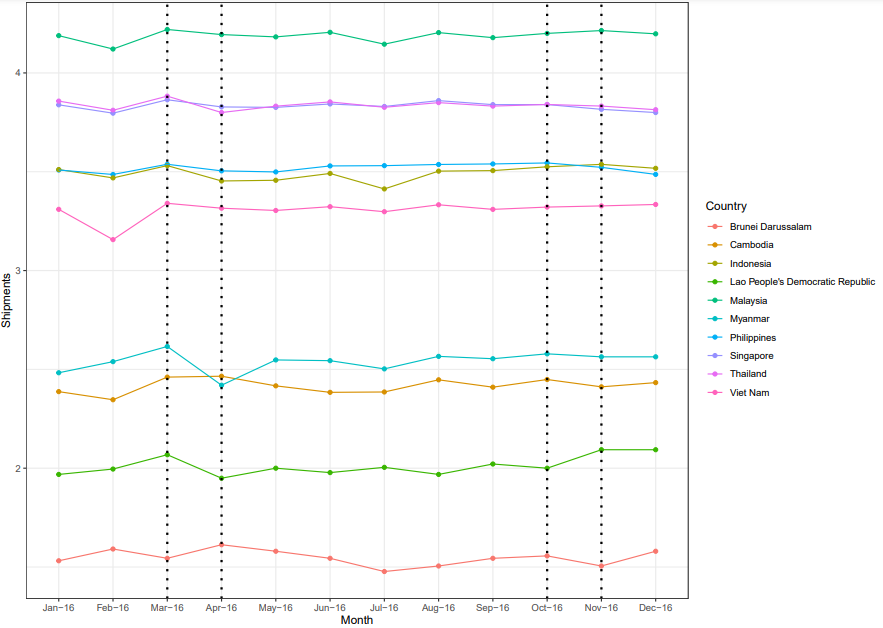
\includegraphics[width=\linewidth]{images/Line Plots/Seasonal/2016_seasonal_log.png}
        \caption{2016 Monthly Shipments, regular and log-scaled (below)}
    \end{minipage}
\end{figure}

\begin{figure}[H]
    \begin{minipage}[c]{1\linewidth}
        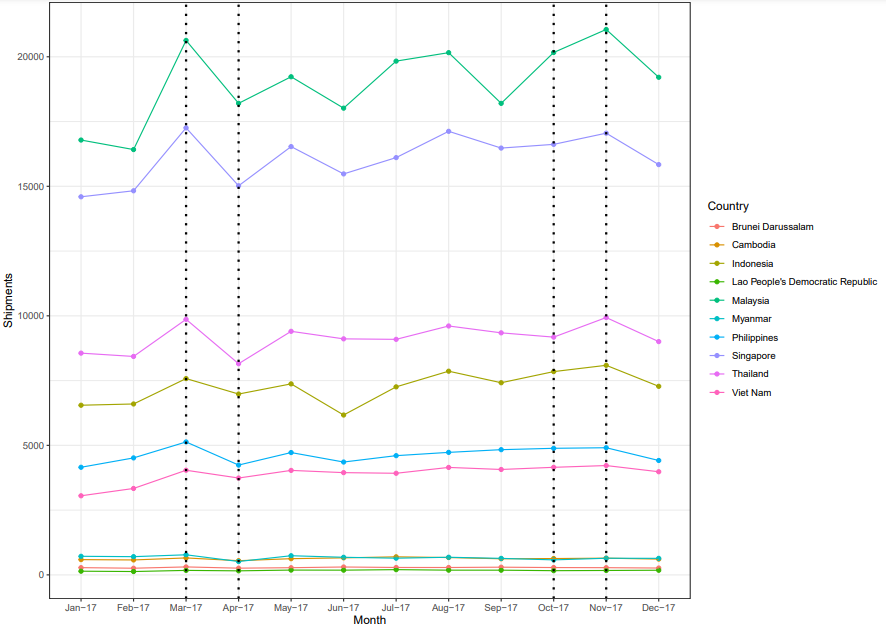
\includegraphics[width=\linewidth]{images/Line Plots/Seasonal/2017_seasonal.png}
    \end{minipage}
    \hfill
    \begin{minipage}[c]{1\linewidth}
        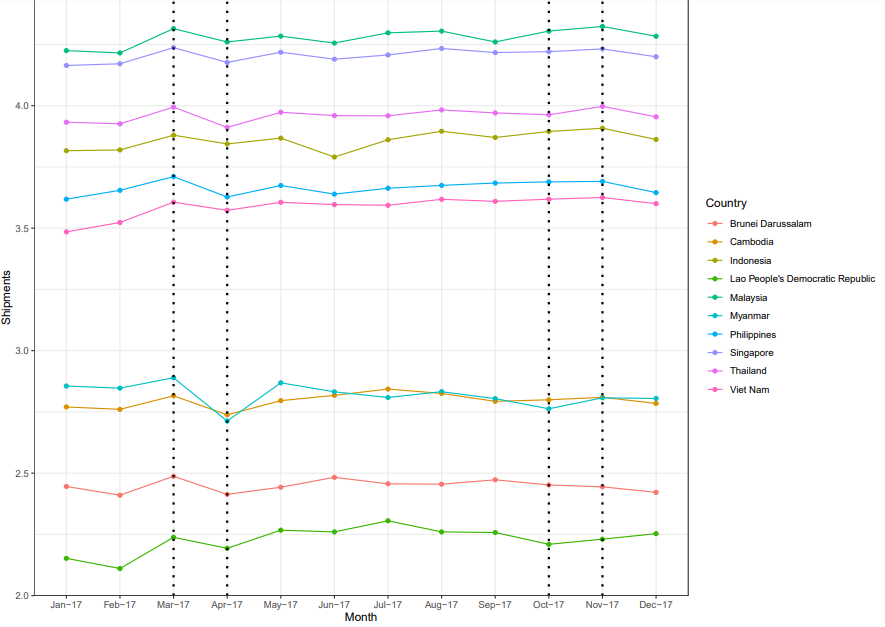
\includegraphics[width=\linewidth]{images/Line Plots/Seasonal/2017_seasonal_log.png}
        \caption{2017 Monthly Shipments, regular and log-scaled (below)}
    \end{minipage}
\end{figure}

\begin{figure}[H]
    \begin{minipage}[c]{1\linewidth}
        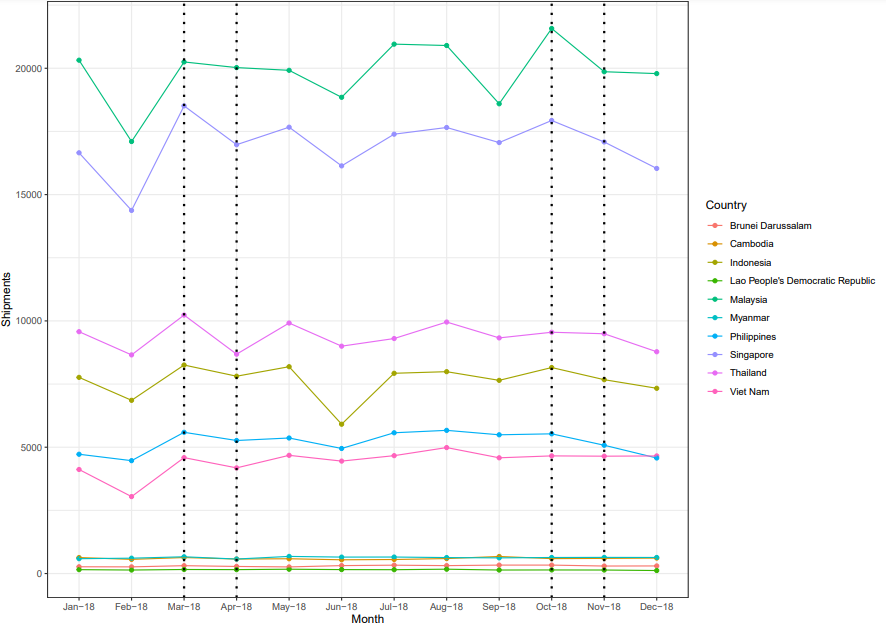
\includegraphics[width=\linewidth]{images/Line Plots/Seasonal/2018_seasonal_log.png}
    \end{minipage}
    \hfill
    \begin{minipage}[c]{1\linewidth}
        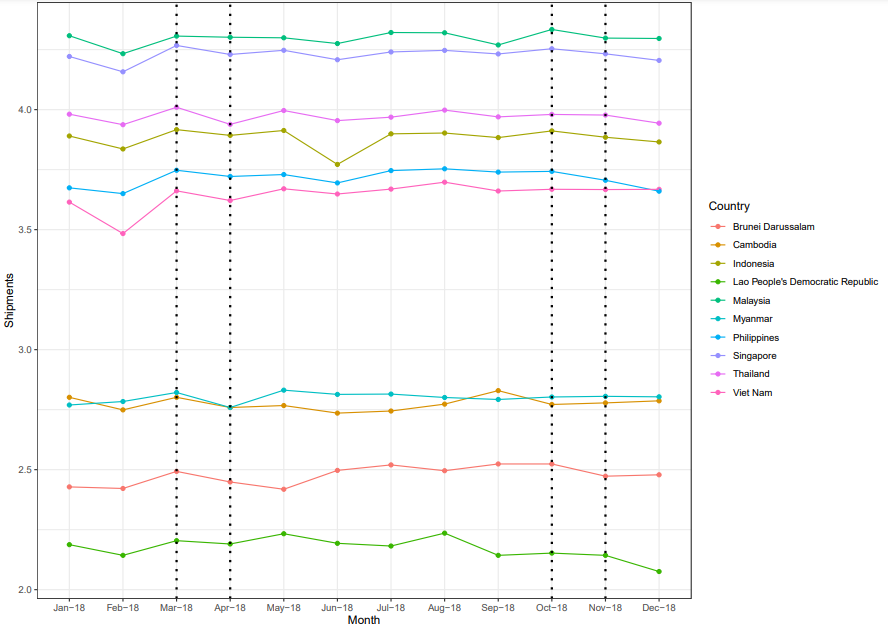
\includegraphics[width=\linewidth]{images/Line Plots/Seasonal/2018_seasonal.png}
        \caption{2018 Monthly Shipments, regular and log-scaled (below)}
    \end{minipage}
\end{figure}

\newpage

\noindent The figures show the presence of a seasonal trend. In general there is a temporary decrease in the number of shipments from March to April, and similarly from October to November, which is consistent throughout each year and each country analysed. This may be due to ... (to be completed)

\newpage

\section{Assessing Macroeconomic Factors of Relevance}

A key challenge of the project involves identifying suitable open-source macroeconomic data relevant to the ASEAN region. In the course of the project, we developed hypotheses about what macroeconomic factors could be of influence on air cargo demand, and how different sets of macroeconomic factors might be related to each other. This will be detailed in the following sections. \\

\noindent There exists a multitude of macroeconomic datasets online, many of which are paywalled or non-accessible to public use without proper licensing. Thus, our identification of relevant macroeconomic data was limited to open-source datasets and those available via existing university subscriptions. The datasets which we accessed were from the following, supplemented by some country's respective department of statistics:

\begin{itemize}
    \item \href{https://data.worldbank.org/}{World Bank Group} 
    \item \href{https://data.imf.org}{International Monetary Fund (IMF)}
    \item \href{https://statista.com}{Statista (Existing Subscription)}
    \item \href{https://tradingeconomics.com/}{Trading Economics}
\end{itemize} 

\subsection{Data Cleaning}
Since we are working with open-source macroeconomic datasets, there is a significant inconsistency in the formatting of each country's datasets. Thus, we had to employ further data cleaning techniques to re-order the data for our use. As we were sourcing for quarterly data, the indicators for each country had to be manually collated into an Excel spreadsheet and reordered based on the given time range.

\subsection{Macroeconomic Indicators}
Our main source of macroeconomic data used is obtained from each country's respective department of statistics, whereby an online open-sourced repository of the country's data is stored. This usually includes the country's National Accounts, as well as data obtained from nation-wide surveys on various indicators such as mean household income. \\

\noindent Some of the macroeconomic indicators which we sourced for initially included the \textit{Balance of Payments (BoP)}, \textit{Gross Domestic Product (GDP)}, \textit{Consumer Price Index (CPI)}, and others such as the \textit{Percentage of Population with Internet Access}. \\

\noindent Each country's department of statistics' portal can be found in the links below:

\begin{multicols}{2}
    \begin{itemize} 
        \item \href{https://www.singstat.gov.sg/}{Singapore}
        \item \href{https://www.data.gov.my/}{Malaysia}
        \item \href{https://www.nesdc.go.th/nesdb_en/main.php?filename=index}{Thailand}
        \item \href{https://psa.gov.ph/}{Philippines}
        \item \href{https://www.bps.go.id/}{Indonesia}
    \end{itemize}
    
    \columnbreak
    
    \begin{itemize}
        \item \href{https://www.gso.gov.vn/en/homepage/}{Vietnam}
        \item \href{https://deps.mofe.gov.bn/Theme/Home.aspx}{Brunei}
        \item \href{https://www.lsb.gov.la/en/home/}{Laos}
        \item \href{https://www.mmsis.gov.mm/}{Myanmar}
        \item \href{https://www.nis.gov.kh/index.php/km/}{Cambodia}
    \end{itemize}

\end{multicols} 

\noindent Where possible, the macroeconomic data sourced was aggregated in quarters, to align with the CargoIS data which was cleaned as aforementioned. 


\subsubsection{Gross Domestic Product} \label{GDP}
GDP, as defined by the IMF, is the monetary value of final goods and services purchased by the user, and produced in a country in a given period of time \cite{GDPdef}. The line plots of each country's raw GDP (at current prices) aggregated in quarters per year is given below, in contrast with their aggregated shipments. Figures are only produced for those countries that provided data on an aggregared quarterly basis (countries that only provided data on an aggregated annual basis are not shown). 

\newpage

\begin{subfigures}
    \begin{figure}[H]
        \centering
        \subfloat[\centering Singapore's Aggregated Shipments]{{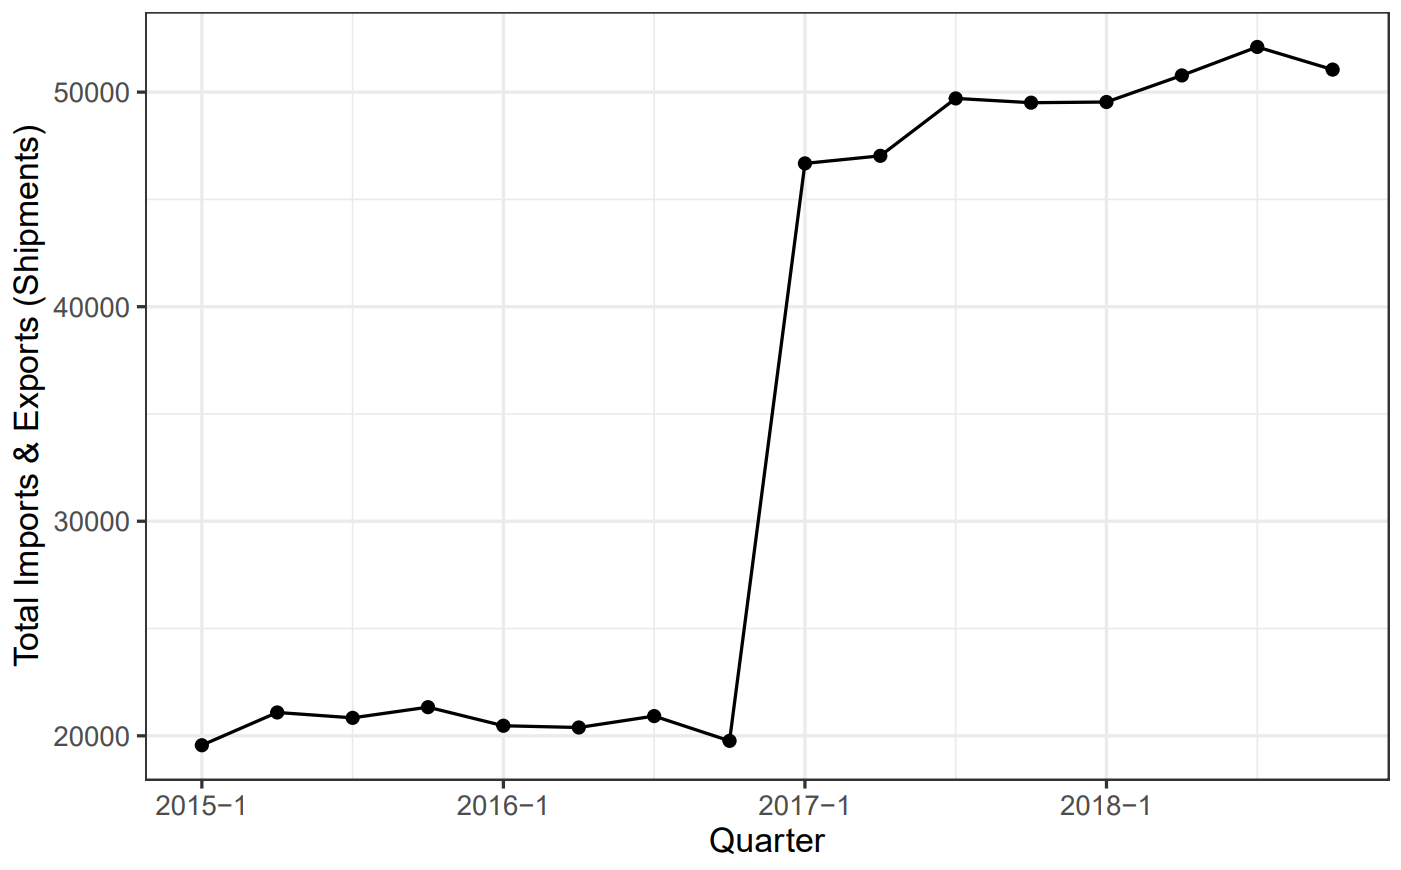
\includegraphics[width=0.47\textwidth]{images/Line Plots/Singapore/SG_Shipments_Quarter.png} }}
        \qquad
        \subfloat[\centering Singapore's GDP]{{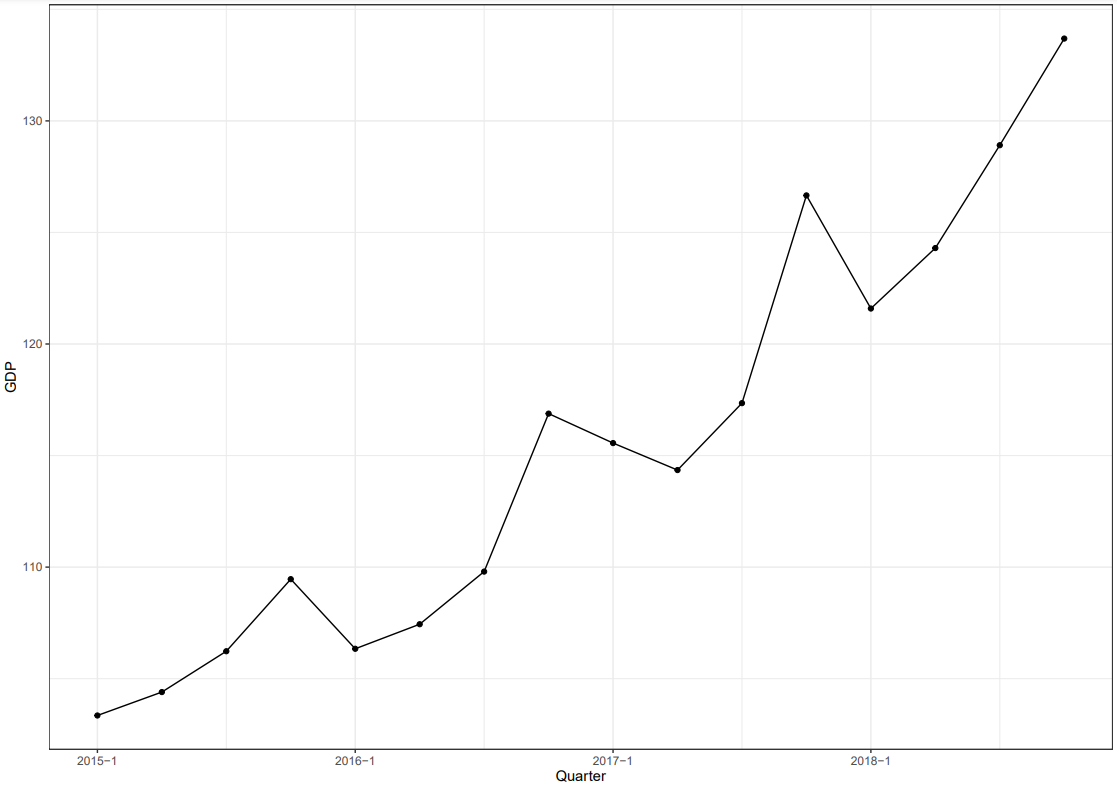
\includegraphics[width=0.45\textwidth]{images/Line Plots/Singapore/SG_GDP_Quarter.png}}}
        \qquad
        \subfloat[\centering Philippines' Aggregated Shipments]{{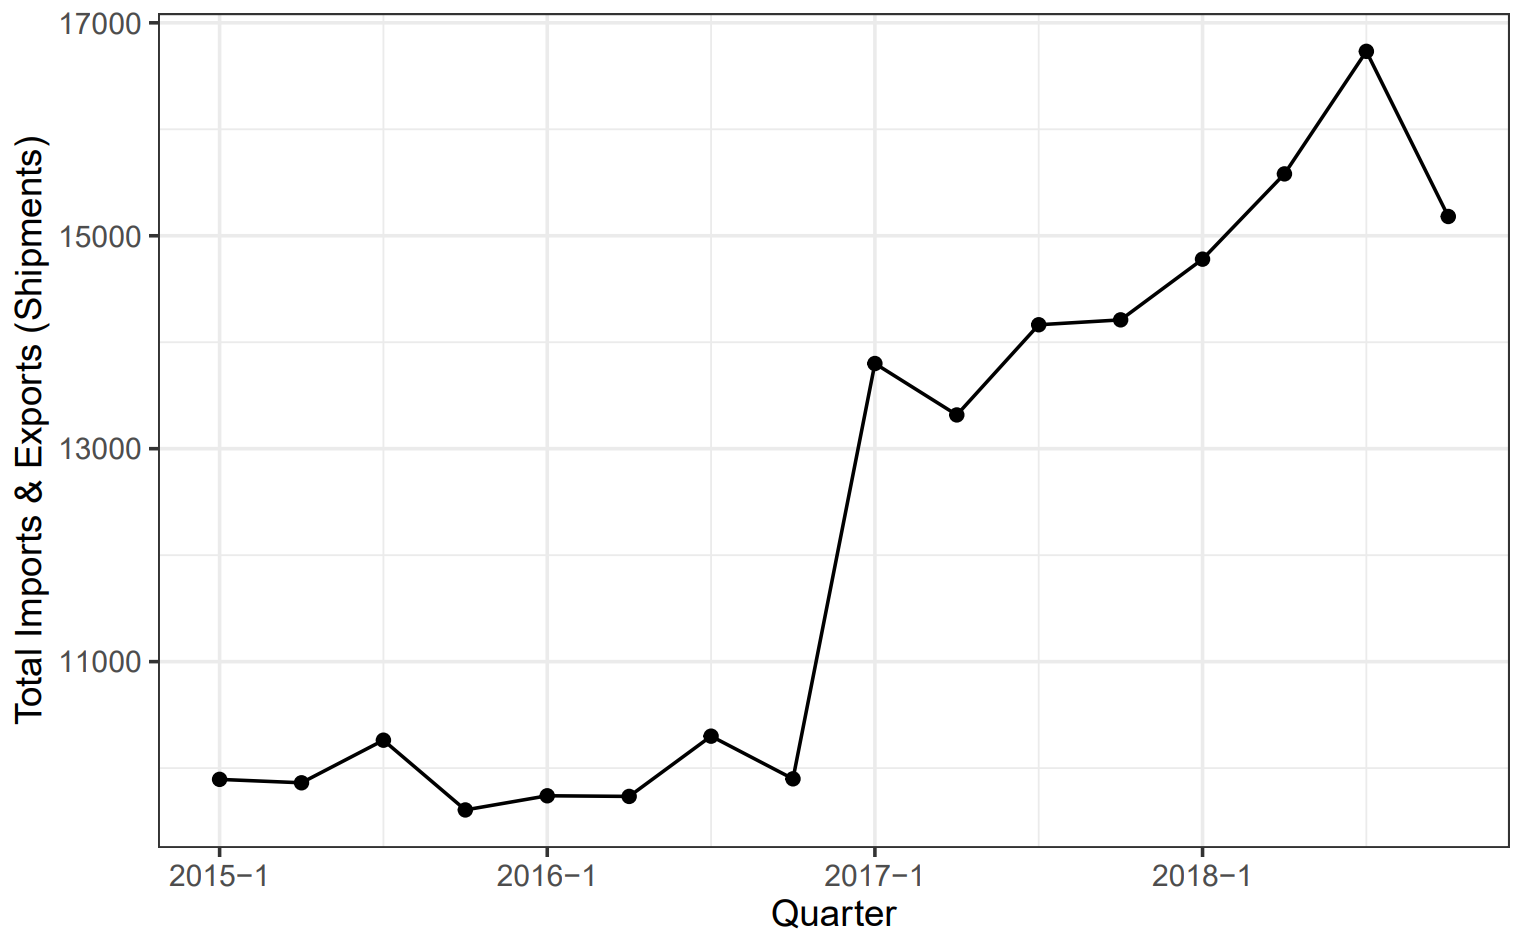
\includegraphics[width=0.47\textwidth]{images/Line Plots/Philippines/PH_Quarterly_Shipments.png} }}
        \qquad
        \subfloat[\centering Philippines' GDP]{{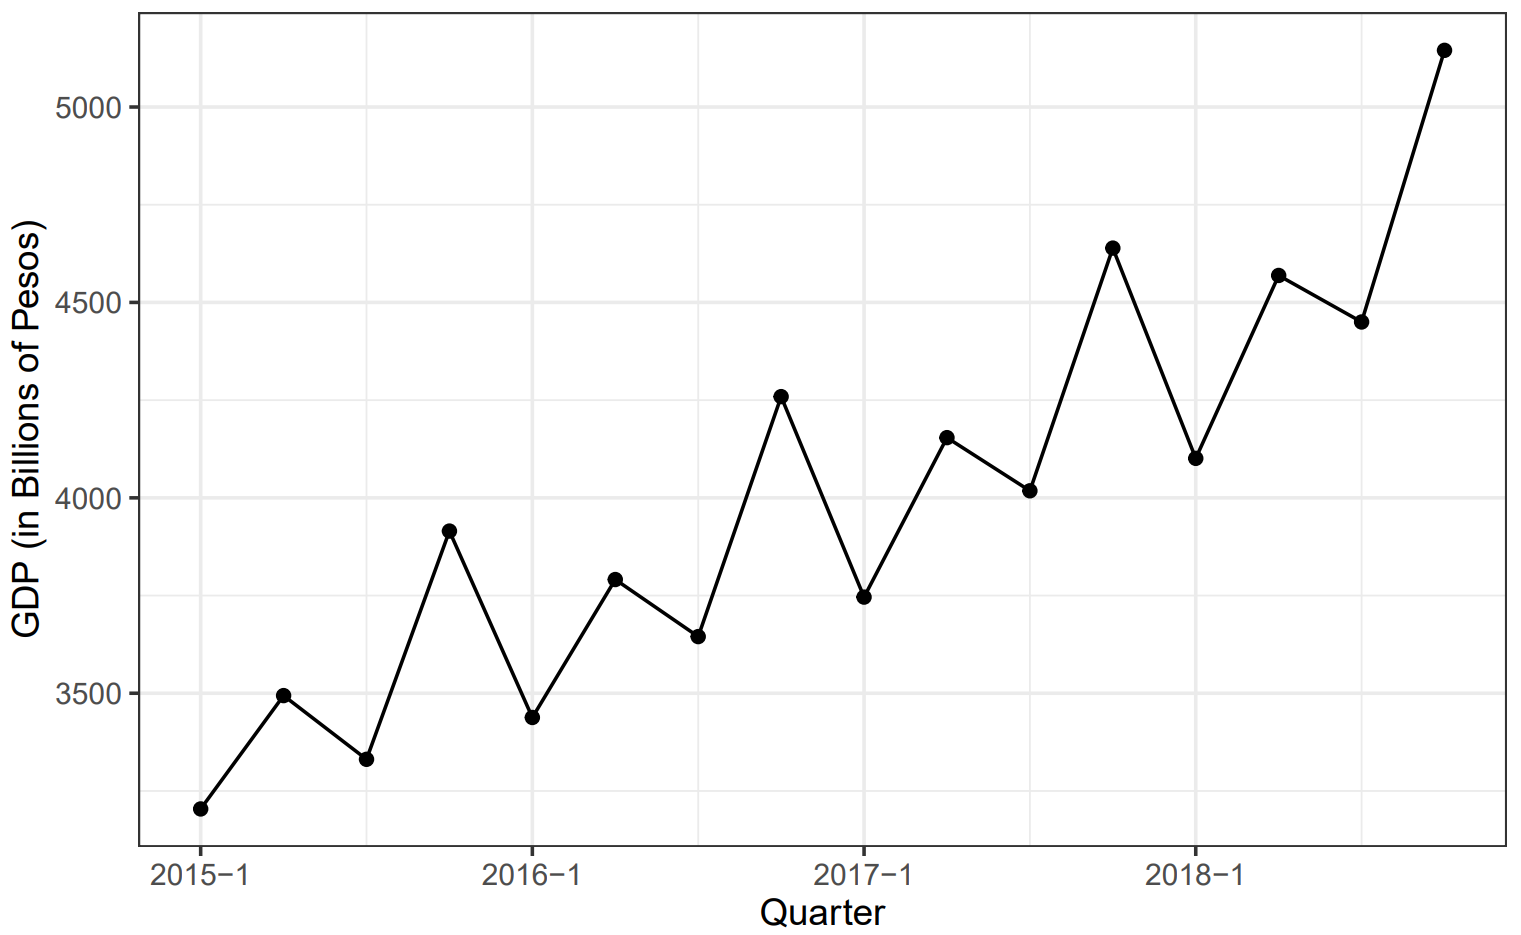
\includegraphics[width=0.47\textwidth]{images/Line Plots/Philippines/PH_Quarterly_GDP.png}}}
        \qquad
        \subfloat[\centering Thailand's Aggregated Shipments]{{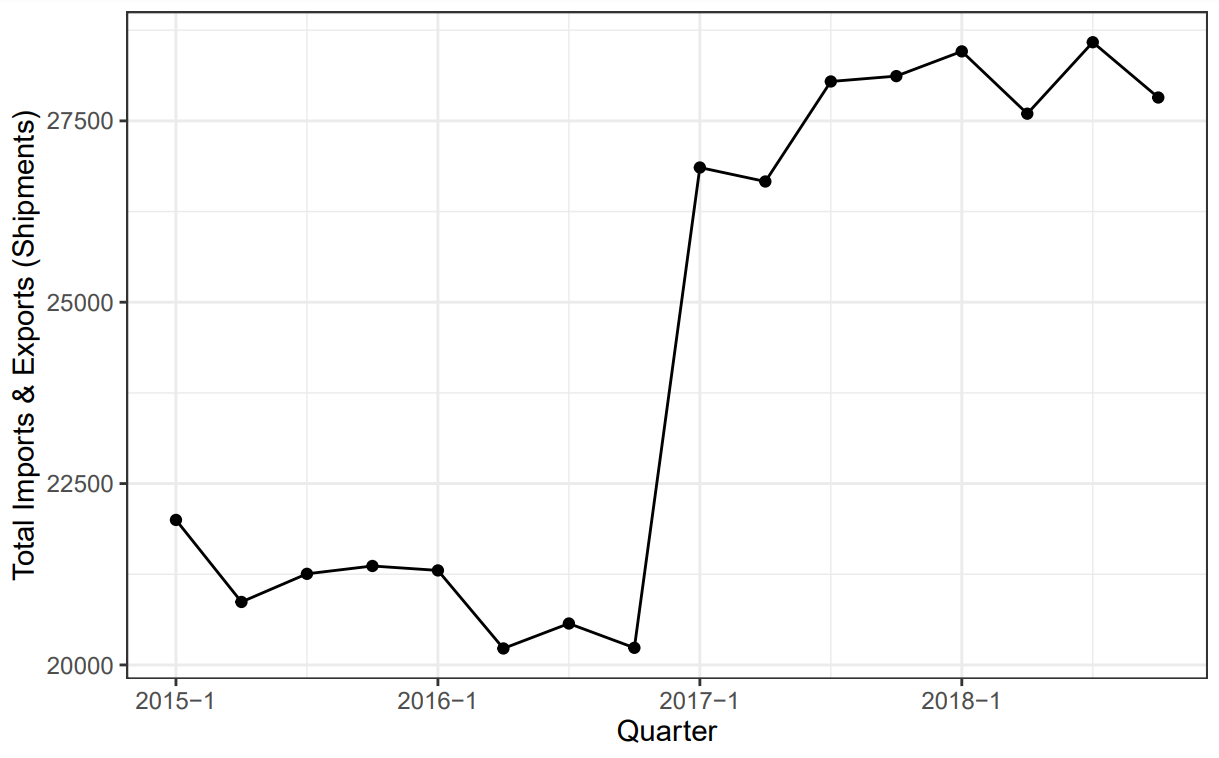
\includegraphics[width=0.47\textwidth]{images/Line Plots/Thailand/Thai_Quarterly_Shipments.png} }}
        \qquad
        \subfloat[\centering Thailand's GDP]{{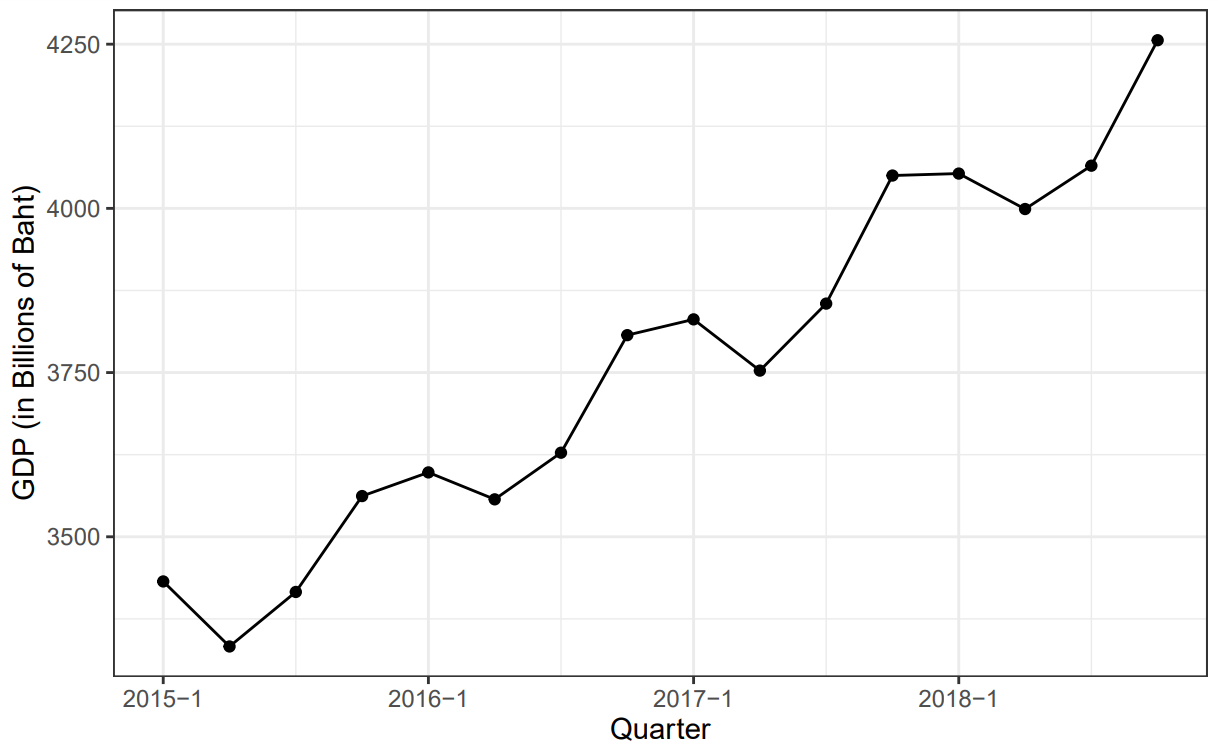
\includegraphics[width=0.47\textwidth]{images/Line Plots/Thailand/Thai_Quarterly_GDP.png}}}
        \caption{Aggregated Shipments and GDP (2015 to 2018)}
    \end{figure}

    \begin{figure}[H]
        \centering
        \subfloat[\centering Malaysia's Aggregated Shipments]{{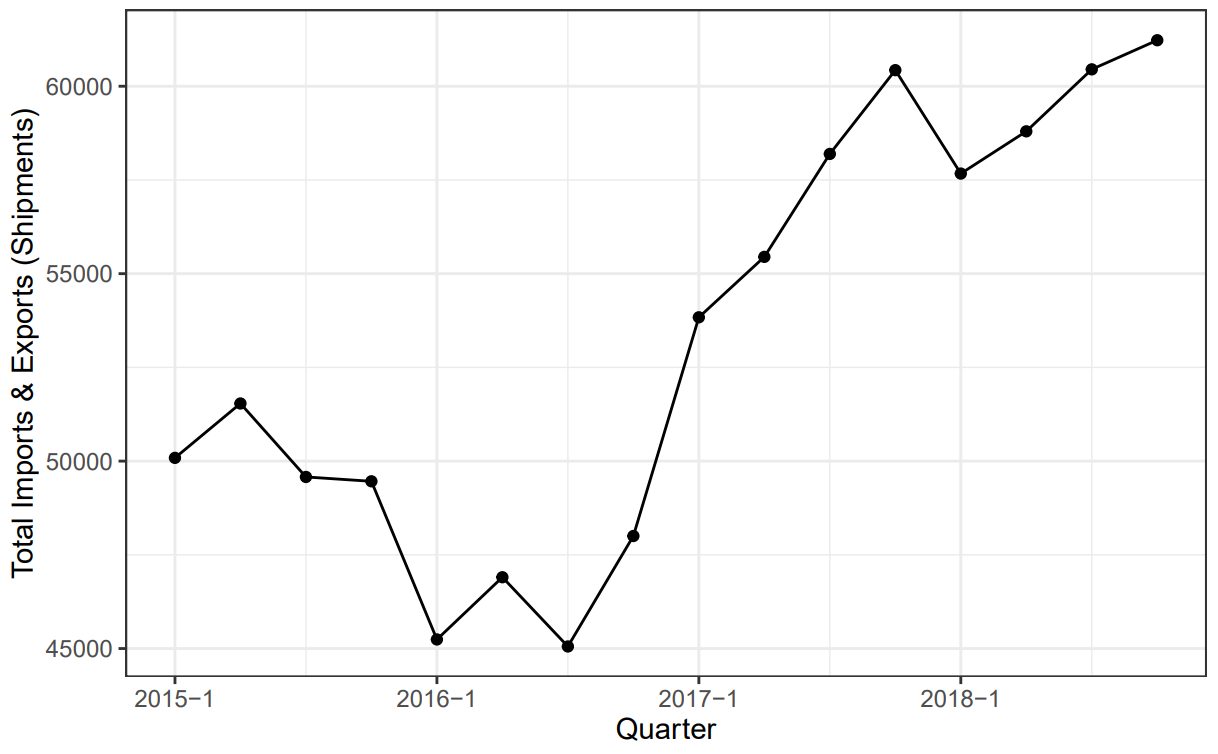
\includegraphics[width=0.47\textwidth]{images/Line Plots/Malaysia/MY_Quarterly_Shipments.png} }}
        \qquad
        \subfloat[\centering Malaysia's GDP]{{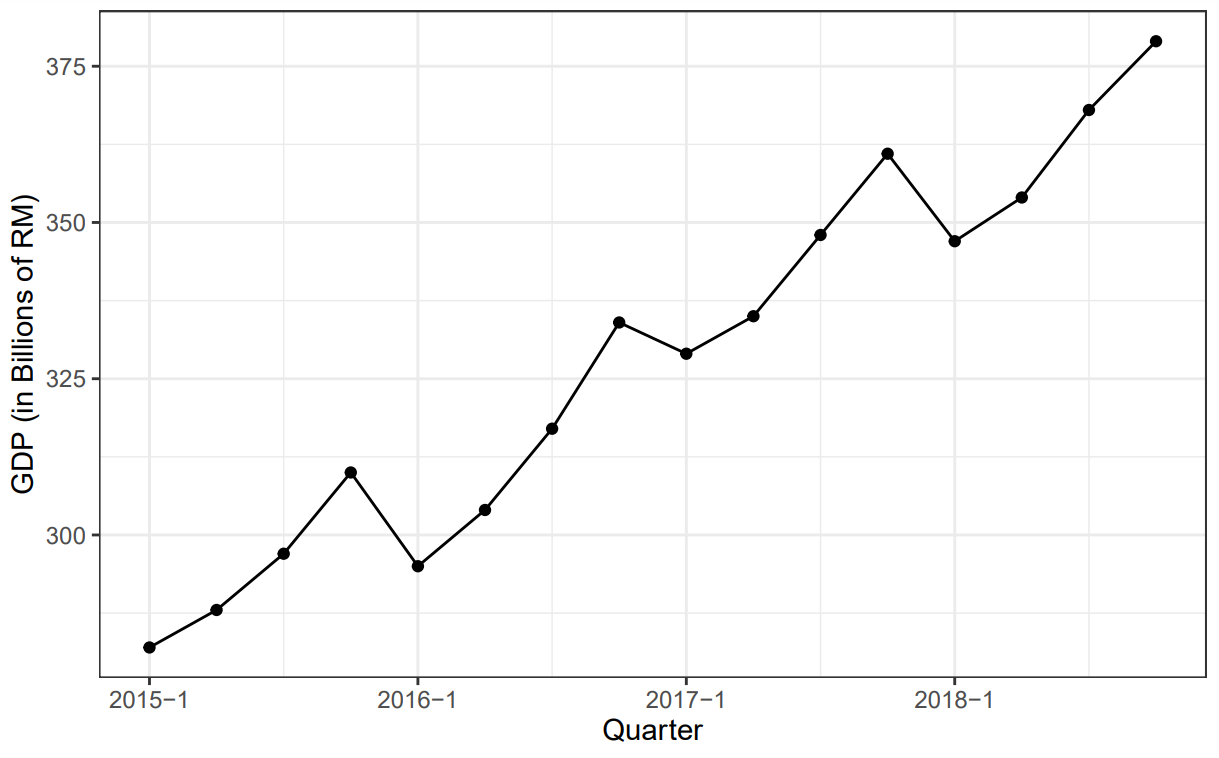
\includegraphics[width=0.47\textwidth]{images/Line Plots/Malaysia/MY_GDP_Quarterly.png}}}
        \qquad
        \subfloat[\centering Indonesia's Aggregated Shipments]{{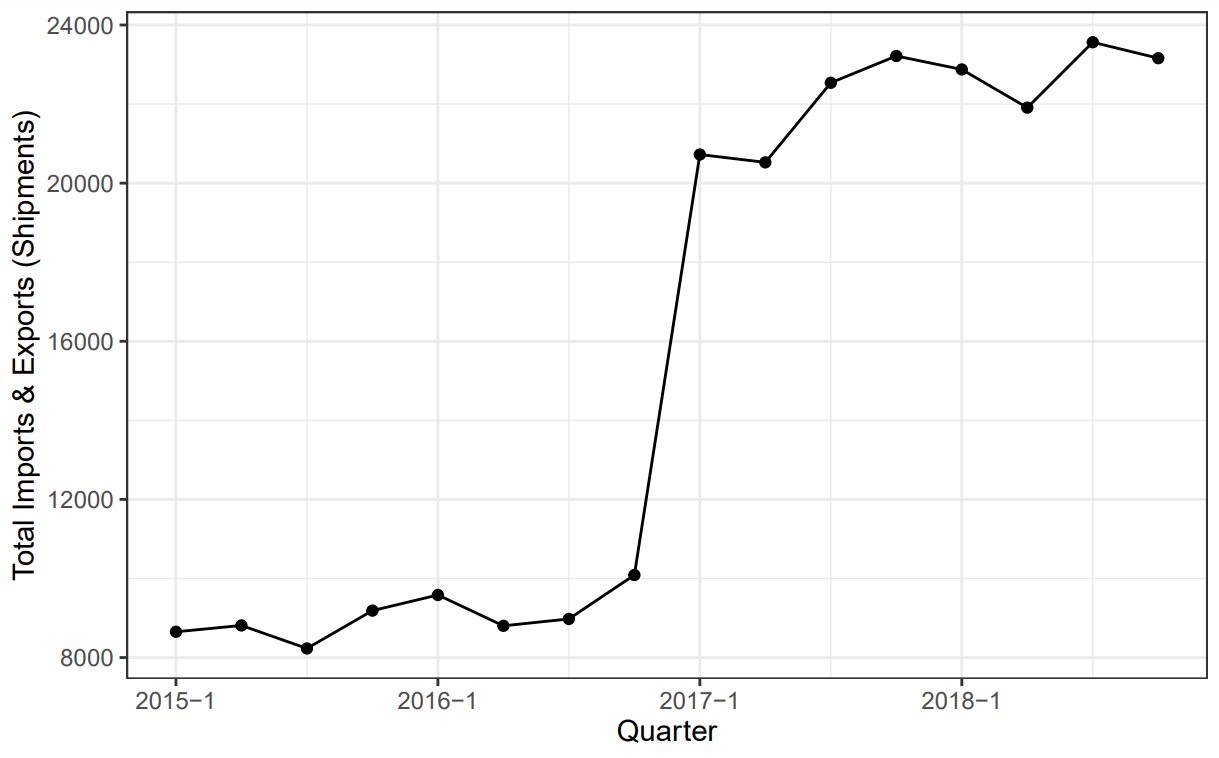
\includegraphics[width=0.47\textwidth]{images/Line Plots/Indonesia/Indonesia_Shipments.png}}}
        \qquad
        \subfloat[\centering Indonesia's GDP (Statista)]{{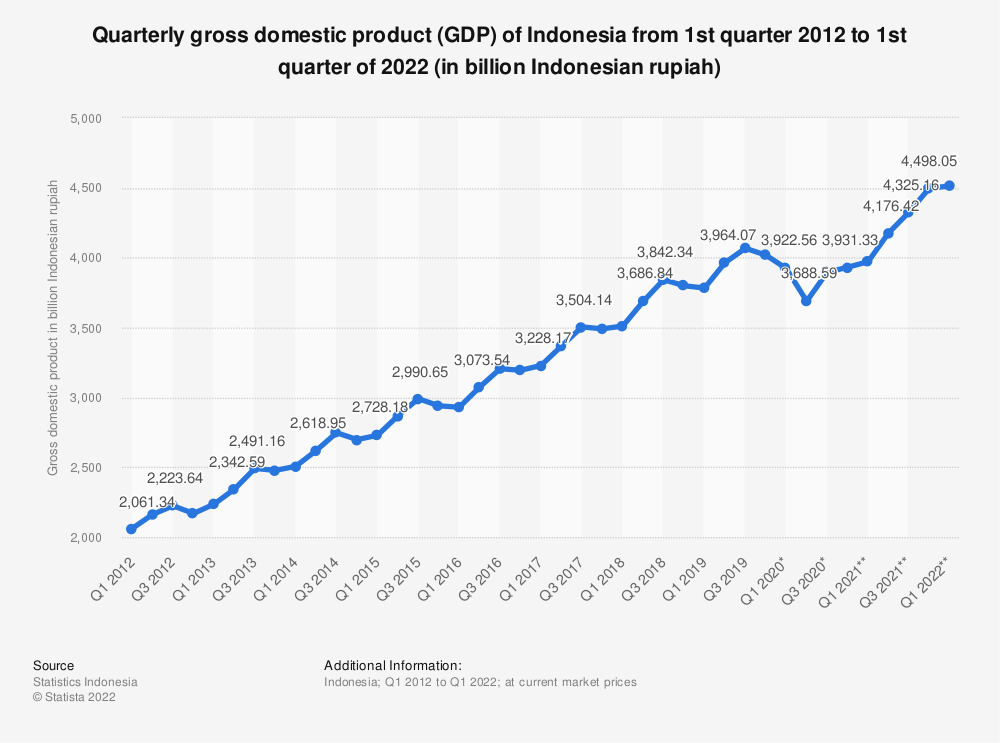
\includegraphics[width=0.47\textwidth]{images/Line Plots/Indonesia/Indonesia_GDP.png}}}
        \qquad
        \subfloat[\centering Brunei's Aggregated Shipments]{{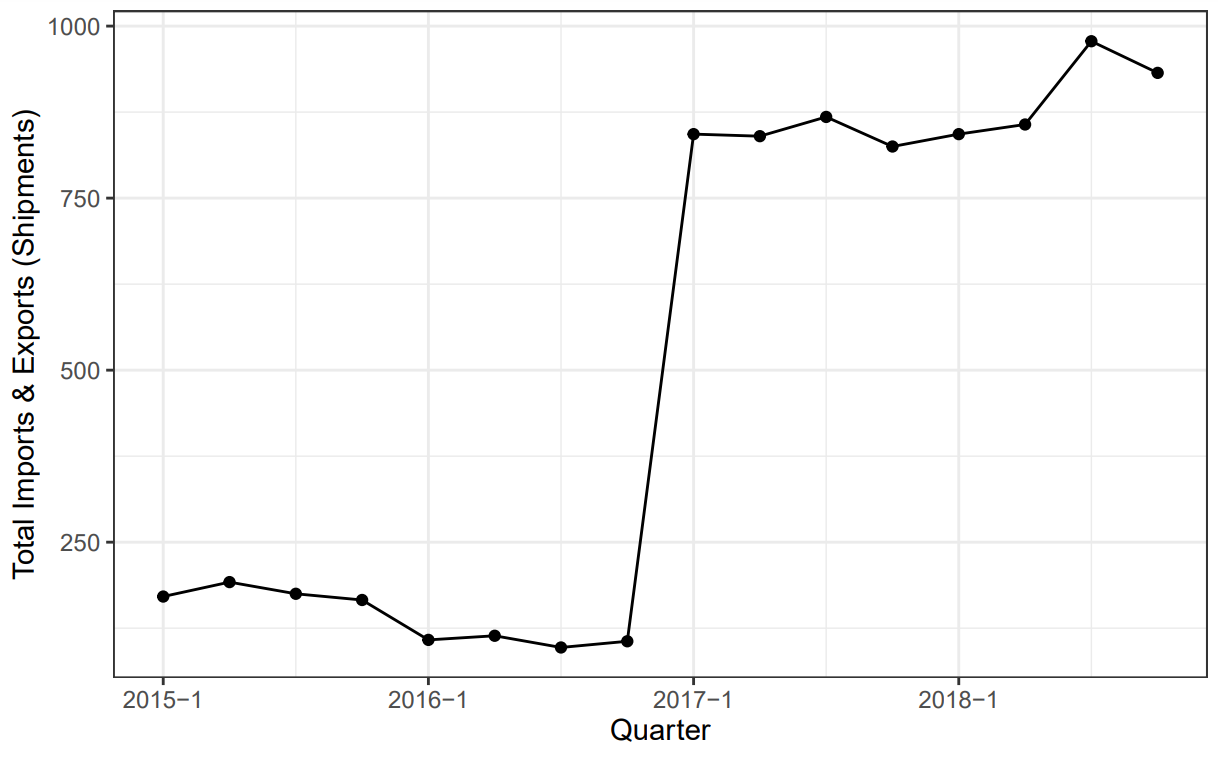
\includegraphics[width=0.47\textwidth]{images/Line Plots/Brunei/Brunei_Shipments_Quarterly.png}}}
        \qquad
        \subfloat[\centering Brunei's GDP]{{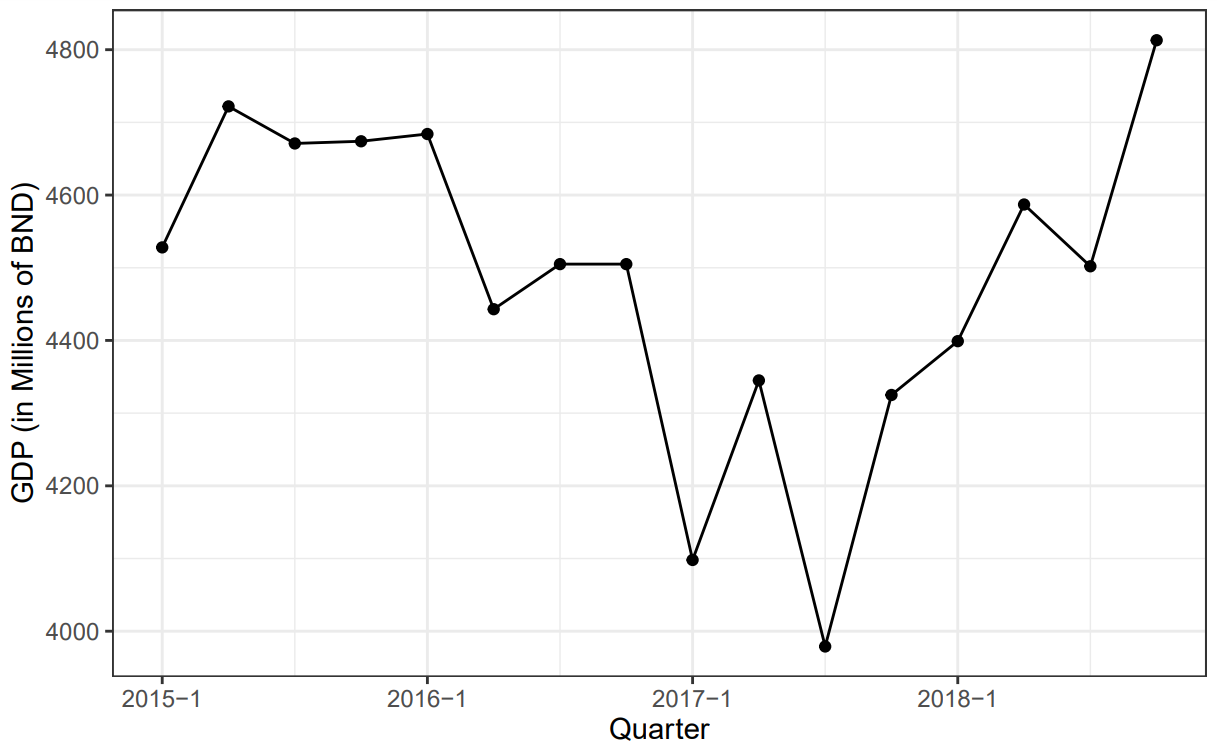
\includegraphics[width=0.47\textwidth]{images/Line Plots/Brunei/Brunei_GDP_Quarterly.png}}}
        \caption{Aggregated Shipments and GDP (2015 to 2018)}
    \end{figure}
\end{subfigures}

% \noindent Aggregate value of the goods and services produced in the economic territory of Singapore. The GDP estimates are compiled based on the output (or production), expenditure and income approaches.

\noindent It can be seen that for most countries, there is a general increase in the GDP over time, whilst the shipments for each country pre-2017 stayed relatively consistent or decreased slightly. Post-2017 however, there seems to be a slight increase over the quarters. Brunei is the only exception to this trend, where its GDP decreased from 2016 to 2017. We suspect this to be due to the oil price collapse in 2016, which largely affected the Brunei economy \cite{BruneiOil}. As a small, oil-rich country, Brunei is heavily dependent on the export of oil and natural gas \cite{Bruneioil2}. Therefore, changes in oil prices can have a significant impact on the country's GDP.

\newpage

% \subsubsection{Government Debt}
% We have also obtained data describing the local government debt of all countries by quarter (ignore first)

% \begin{figure}[H]
% \centering
% 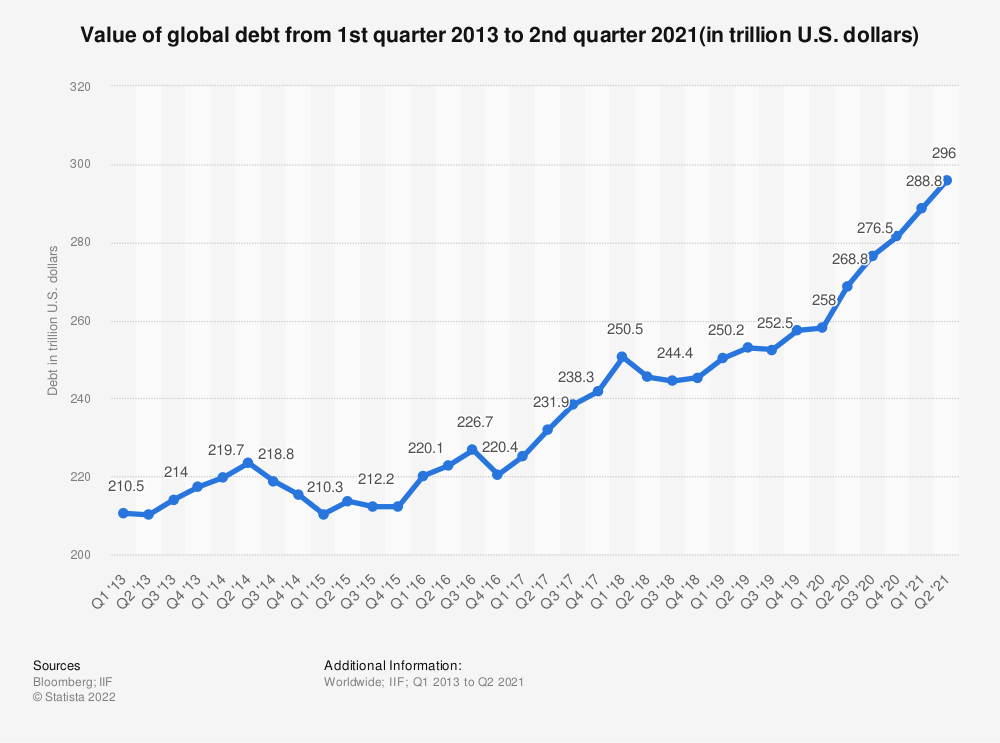
\includegraphics[width=0.8\textwidth]{images/Line Plots/Global Debt/Global_Debt.png}
% \caption{\label{fig2}Global Debt Values}
% \end{figure}

\subsection{Correlation of Air Cargo Data with Macroeconomic Data}

As our dataset is too small to conduct meaningful regression analysis, we decided to proceed with correlation analysis with the given 16 data points. 

\subsubsection{Pearson's Correlation Coefficient}
The Pearson's Correlation Coefficient is a statistical measure of linear correlation between two sets of data. Mathematically, it is the covariance of the two variables divided by the product of their standard deviations. When applied to a sample with bivariate data of $n$ pairs, the formula is given by \\

\begin{equation}
    r = \frac{ \sum_{i=1}^{n}(x_i-\bar{x})(y_i-\bar{y}) }{%
        \sqrt{\sum_{i=1}^{n}(x_i-\bar{x})^2}\sqrt{\sum_{i=1}^{n}(y_i-\bar{y})^2}}
\end{equation} \\

\noindent The correlation coefficient ranges from $-1$ to $1$. An absolute value of exactly $1$ implies that a linear equation describes the relationship between $X$ and $Y$ perfectly, while the sign denotes positive or anti-correlation. Values of r close to zero indicates little to no linear correlation. \\

\noindent Correlation plots (Pair Plots in $R$) are shown below, between the macroeconomic indicator and the number of shipments of each country, along with the Pearson's correlation value in the upper right matrix. The statistical significance of the correlation value will be expanded on in section \ref{HypoTest}. Plots along the diagonal represent the density distribution plot of the number of shipments or GDP correspondingly. These plots are obtained via kernel density estimates to show the probability density function of each variable and are essentially smoothed-out histogram plots. The peaks of the distribution displays where values are concentrated over the interval. \\

\begin{figure}[H]
    \centering
    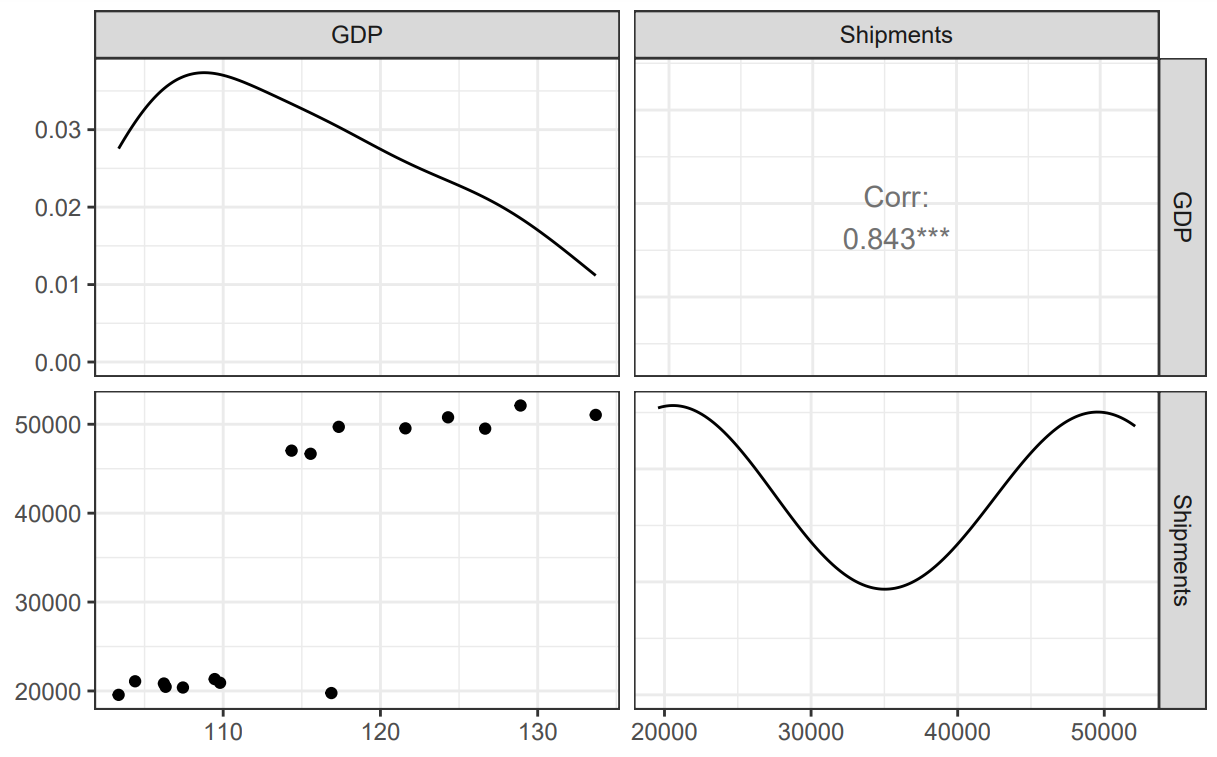
\includegraphics[width=1\textwidth]{images/Line Plots/Singapore/Singapore_Corrplot.png}
    \caption{Singapore GDP Correlation Plot}
    \label{fig:my_label}
\end{figure}

\begin{figure}[H]
    \centering
    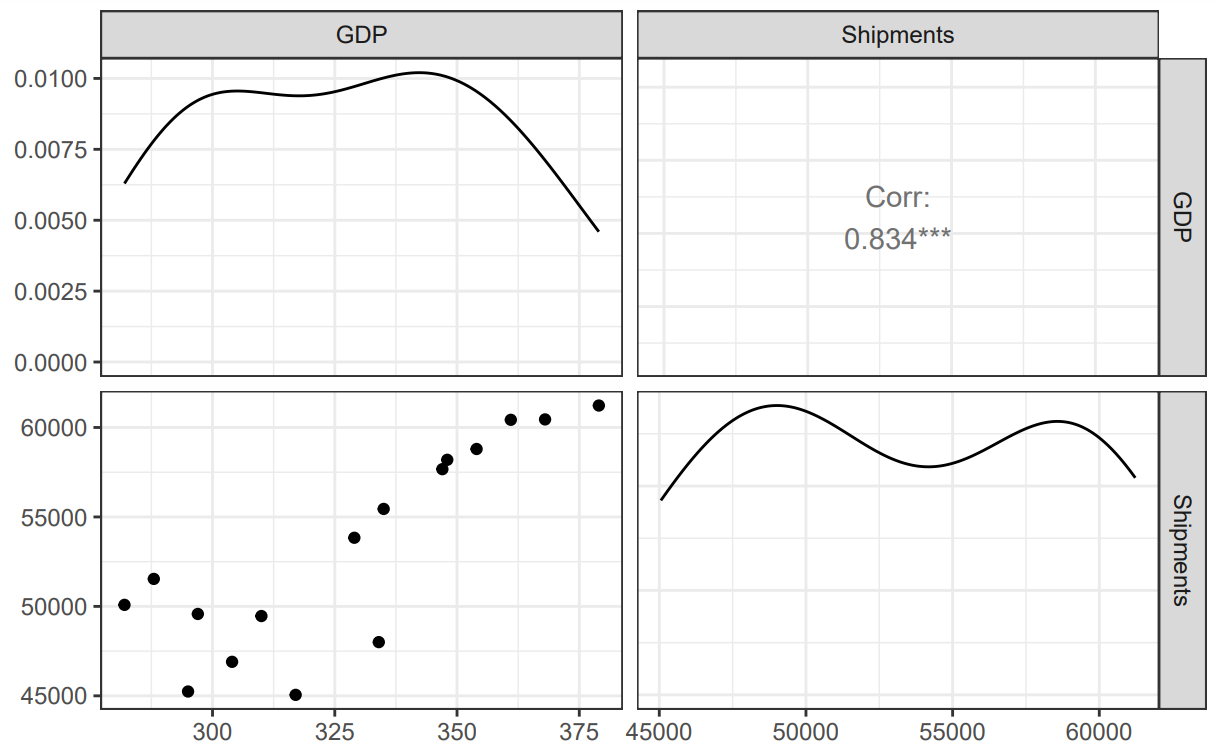
\includegraphics[width=1\textwidth]{images/Line Plots/Malaysia/Malaysia_Corrplot.png}
    \caption{Malaysia GDP Correlation Plot}
    \label{fig:my_label}
\end{figure}

\begin{figure}[H]
    \centering
    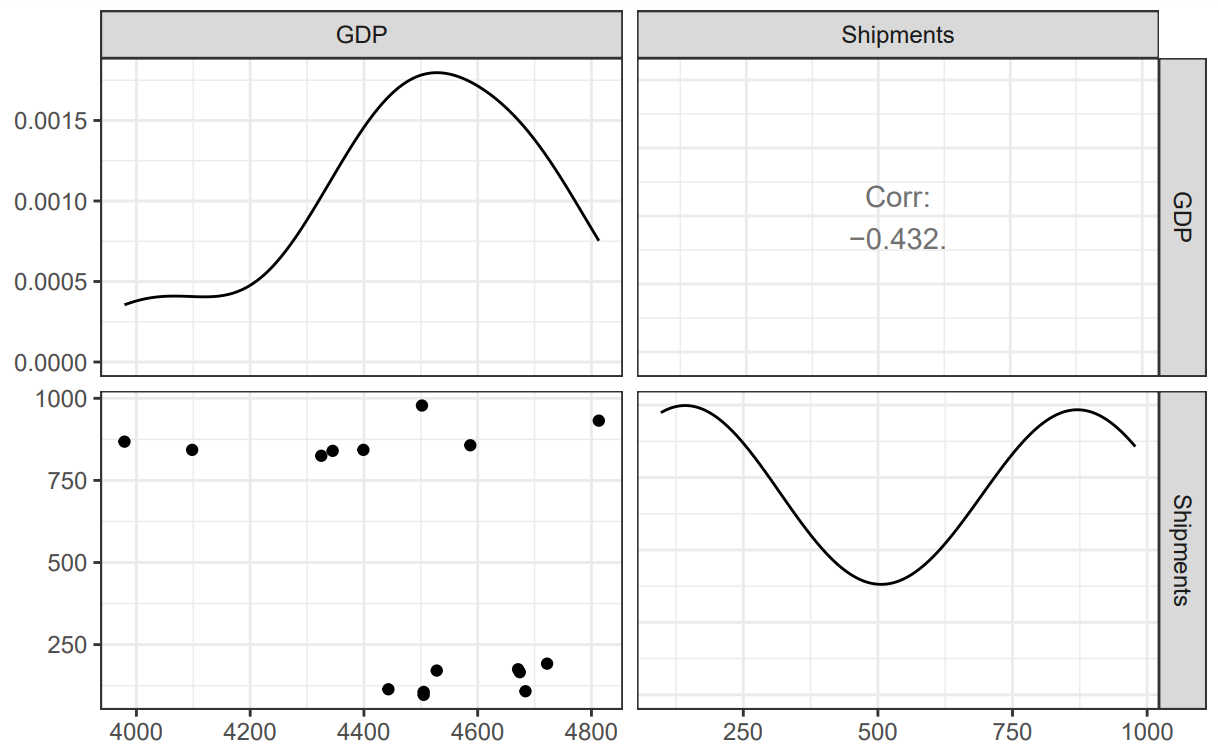
\includegraphics[width=1\textwidth]{images/Line Plots/Brunei/Brunei_Corrplot.png}
    \caption{Brunei GDP Correlation Plot}
    \label{fig:my_label}
\end{figure}

\begin{figure}[H]
    \centering
    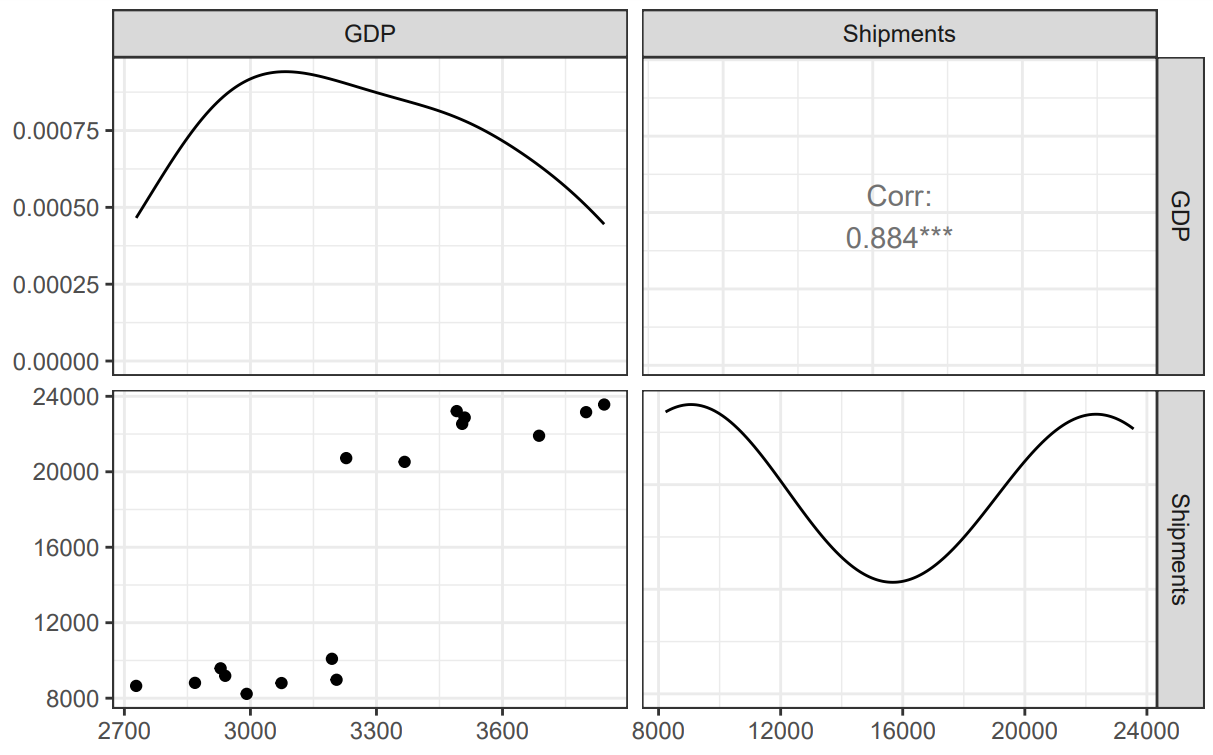
\includegraphics[width=1\textwidth]{images/Line Plots/Indonesia/Indonesia_Corrplot.png}
    \caption{Indonesia GDP Correlation Plot}
    \label{fig:my_label}
\end{figure}

\begin{figure}[H]
    \centering
    \includegraphics[width=1\textwidth]{images/Line Plots/Philippines/Philippines_Corrplot.png}
    \caption{Philippines GDP Correlation Plot}
    \label{fig:my_label}
\end{figure}

\begin{figure}[H]
    \centering
    \includegraphics[width=1\textwidth]{images/Line Plots/Thailand/Thailand_Corrplot.png}
    \caption{Thailand GDP Correlation Plot}
    \label{fig:my_label}
\end{figure}

\noindent Notable trends include the similar shape of each density distribution of the shipments for all countries, which indicates that most countries tend to either engage in trade with very large or small number of shipments, but little in-between. \\

\noindent Another interesting observation is the \textit{relatively} high correlation values for each country (excluding Brunei), suggesting possibly a correlation between the GDP values of a country and its corresponding number of shipments, reemphasizing the observation found in section \ref{GDP}.

\subsubsection{Hypothesis Testing} \label{HypoTest}
For us to determine whether the correlation values are statistically significant, we employed hypothesis testing on the correlation coefficient obtained. To measure the significance of our empirical analyses, we used the \textbf{\textit{p-value}}, which is defined as the probability of obtaining results ‘as extreme’ or ‘more extreme’, under the assumption that the null hypothesis is true. The lower the p-value, the higher the significance of our obtained correlation coefficient. We used \textit{R}'s in-built correlation test function with the standard significance level $\alpha = 0.05$ to determine the respective p-values of each observation, as shown below. The function returns a list of statistics: The \textit{t} test statistic, degrees of freedom, p-value, and the correlation value. 

\begin{center}
\begin{tabular}{ |c|c|c|c|c| } 
 \hline
    \textit{\textbf{Country}} & \textit{\textbf{t}} & \textit{\textbf{d.o.f}} & \textit{\textbf{p-value}} & \textit{\textbf{Correlation Value}} \\
    \hline
    Singapore & $5.8576$ & $14$ & $\num{4.163e-05}$ & $0.8427438$  \\
    \hline
    Malaysia & $5.6571$ & $14$ & $\num{5.917e-05}$ & $0.8340666$ \\
    \hline
    Brunei & $-1.7915$ & $14$ & $\num{.09485}$ & $-0.4318419$  \\
    \hline
    Indonesia & $7.0863$ & $14$ & $\num{5.453e-06}$ & $0.8843$  \\
    \hline
    Philippines & $4.0627$ & $14$ & $\num{.001164}$ & $0.7355751$  \\
    \hline
    Thailand & $5.6467$ & $14$ & $\num{6.027e-05}$ & $0.8336006$  \\
    \hline
\end{tabular}
\end{center} 

\noindent We can observe from the statistics obtained that the \textit{p-values} of Singapore, Malaysia, Indonesia, Philippines, and Thailand, are lower than the significance level $\alpha$. This indicates a strong evidence to reject our null hypothesis, which means that our results obtained for the correlation values are statistically significant. The \textit{p-value} for Brunei however, is greater than $\alpha$, which indicates a strong evidence for the null hypothesis, that there is no statistical correlation between Brunei's GDP and the total number of shipments per quarter. \\

\noindent Despite most countries showing correlation between GDP and the number of shipments however, this does not necessarily imply direct causation, as air cargo demand is still influenced by many other factors. It is also important to note that although the \textit{p-value} may be low, this does not immediately indicate that our null hypothesis is false. Rather, it means that the observed result is unlikely to have occurred by chance and warrants further investigation.

\section{Conclusions}
Throughout the course of this project, we have conducted analysis on the various macroeconomic factors that influence the demand for air cargo within ASEAN.

\subsection{Further Recommendations}
We recommend that additional studies should be conducted to explore more factors that might influence air cargo demand within ASEAN countries, including non-macroconomic indicators. These factors of significance should also be further tested for reliability before being employed for statistical analysis. Furthermore, unlike common data science pipelines used in the industry, one core limitation of our project involves the manual sourcing of open-source datasets online, which is generally time consuming and prone to human error. Further studies conducted, where possible, should consider the use of techniques such as web-scraping and APIs integrated within their pipeline to extract business insights. Lastly, another limitation of this project was the insufficient data used in conducting statistical analysis, which may affect the reliability of our obtained values. Further studies conducted should consider obtaining more data before embarking on any statistical analysis. 

\section*{Acknowledgements}
This research is supported in part by grant RS-CAASI-00009 from the Civil Aviation Authority of Singapore (CAAS), and the International Air Transport Association for providing access to the air cargo dataset. We would also like to thank Professor Peter Jackson (Institute Director, ASI), and Jamie Bloomfield, (Lead, Translational Research and Industry Engagement, ASI), for their unwavering support and for providing invaluable advice throughout the course of this project. 

\bibliographystyle{apacite}
\bibliography{refs}

\end{document}